\documentclass{article}

% if you need to pass options to natbib, use, e.g.:
%     \PassOptionsToPackage{numbers, compress}{natbib}
% before loading neurips_2020

% ready for submission
% \usepackage{neurips_2020}

% to compile a preprint version, e.g., for submission to arXiv, add add the
% [preprint] option:
%     \usepackage[preprint]{neurips_2020}

% to compile a camera-ready version, add the [final] option, e.g.:
%     \usepackage[final]{neurips_2020}

% to avoid loading the natbib package, add option nonatbib:
\usepackage[preprint]{neurips_2020}

\usepackage[utf8]{inputenc} % allow utf-8 input
\usepackage[T1]{fontenc}    % use 8-bit T1 fonts
\usepackage{hyperref}       % hyperlinks
\usepackage{url}            % simple URL typesetting
\usepackage{booktabs}       % professional-quality tables
\usepackage{amsfonts}       % blackboard math symbols
\usepackage{nicefrac}       % compact symbols for 1/2, etc.
\usepackage{microtype}      % microtypography

\usepackage{graphicx}               % For adding images from file
\graphicspath{ {./report_images/} } % Directory having all images

\usepackage{caption}        % to add images in figures
\usepackage{subcaption}     % to add images as subfigures

\title{Evaluating and Visualizing the properties of Dropout for GRU}

% The \author macro works with any number of authors. There are two commands
% used to separate the names and addresses of multiple authors: \And and \AND.
%
% Using \And between authors leaves it to LaTeX to determine where to break the
% lines. Using \AND forces a line break at that point. So, if LaTeX puts 3 of 4
% authors names on the first line, and the last on the second line, try using
% \AND instead of \And before the third author name.

\author{%
  Amit Hattimare, Rachana Acharya \\
  University of Massachusetts, Amherst \\
  \texttt{\{ahattimare,rnacharya\}@umass.edu} \\
  % examples of more authors
  % \And
  % Rachana Acharya \\
  % \texttt{rnacharya@umass.edu} \\
  % \AND
  % Coauthor \\
  % Affiliation \\
  % Address \\
  % \texttt{email} \\
  % \And
  % Coauthor \\
  % Affiliation \\
  % Address \\
  % \texttt{email} \\
  % \And
  % Coauthor \\
  % Affiliation \\
  % Address \\
  % \texttt{email} \\
}

\begin{document}

\maketitle

\begin{abstract}
  Dropout technique in all its variations is known to improve generalization performance for multi-layer perceptron and CNN based models. There has been work to show how introduction of dropout and choosing the right hyperparameters change the loss landscape, and make it easier to reach covergence. Dropouts have also been successfully applied on RNN based models but their reason for performance improvement has not been studied visually. In this paper, we apply zoneout and dropconnect dropouts on GRU based models for analysing a sentiment classification problem and reason the performance based on model convergence and changes in the loss landscape. We use "filter normalization" technique to perform dimensionality reduction and get 2D and 3D loss surface visualizations. We tune the hyperparameters and compare the best models with and without dropouts. We see that introduction of dropout increases the area having minimum loss indicating that the number of optimal weight combinations increases. We notice the confidence on the predictions going up in some cases, which suggests that dropout, while increasing optimum parameters range, generalizes better on the test data. We also evaluated the robustness of dropout with respect to adversarial inputs and found that models trained with DropConnect perform significantly better in comparison to the baseline model without dropout. 
\end{abstract}

\section{Introduction}
Dropout is a well known regularization method that has been very successful with all kinds of feed-forward neural networks. Its properties have been well studied for image based neural networks. However, the reasons for its performance improvements on recurrent neural network based models, such as its effect on the underlying loss landscape and its resilience to noisy inputs have not been studied. This project aims to understand these aspects of some popular dropout techniques for a recurrent neural network model using Gated Recurrent Unit(GRU) cells. 

\section{Novelty Statement}
\cite{li2018visualizing} describes the effect on the loss landscape of some of the popular image based models such as VGG, ResNet and DenseNet using visualizations. There has been a lot of work understanding certain other properties of dropout for example co-adaptation of weights, dropout penalty, averaging and regularizing property, etc. Simple neural networks were studied in \cite{DBLP:journals/corr/HelmboldL16} and deep neural networks in \cite{conf/nips/BaldiS13}, among others. But, we do not see any related work in understanding the effects of dropout on the loss landscape of different models. Moreover, dropout has been relatively less understood in the area of recurrent neural networks (RNN) owing to the fact that there could be a loss of memory when we drop activations of hidden units. There has been application of new dropout techniques such as Variational dropout \cite{gal2016theoretically}, Zoneout \cite{krueger2017zoneout}, and Recurrent Dropout \cite{semeniuta2016recurrent} on RNNs but the effect has been studied only with respect to accuracy and convergence. Other properties such as the dropout variant's ensemble averaging, co-adaption of weights, the dropout penalty with respect to various forms of regularization techniques have not been studied. We specifically look into a GRU based model and study the effects of Zoneout and Dropconnect \cite{pmlr-v28-wan13} on model convergence, loss landscape visualization and resilience towards adversarial inputs using sentiment analysis of the IMDB movie review dataset.

\begin{figure}[h]
	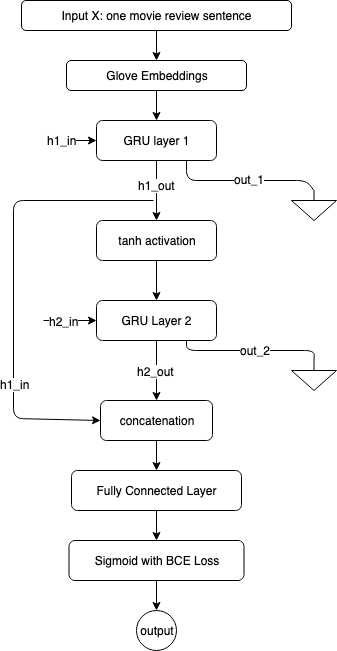
\includegraphics[scale=0.5]{gru_model_architecture.png}
	\centering
	\caption{Architecture diagram for 2 layer GRU model.}
	\label{fig:gru_model}
\end{figure}

\section{Related work}
A lot of recent work has been done in the parameter and loss visualization space but mostly for image classification tasks. \cite{li2018visualizing} paper visualizes the effect on loss landscape of neural networks due to skip connections, increased number of hidden layers using SGD optimization. \cite{NIPS2018_7515} paper visualizes the effects of batch normalization(BN) on neural network properties and concludes that BN does not contribute to internal covariance shift but rather makes the optimization problem smooth.

\cite{neal2019modern} paper studies the bias-variance curve as a function of Neural Network complexity and shows that both bias and variance and go down simultaneously as the model complexity increases. Again, through visualization and mathematical modeling, \cite{yang2020rethinking} paper indeed showed that as model complexity increases in NN, bias always down but variance shows a bell-like curve.

\cite{gal2016theoretically} paper applies Dropouts on GRU for movie review task and proposes a novel way of applying dropout ratios on GRU connections. Performance is simply compared using error rates on the test data without other visualizations. 

\cite{DBLP:journals/corr/abs-1809-05165} talk about applying dropout at test time to check the robustness of image based Deep Neural Networks. The technique is called as Defensive Dropout. We apply this technique to our GRU model to check the robustness of the model against adversarial inputs.

\cite{morris2020textattack} introduce a Python framework for adversarial attacks, adversarial training, and data augmentation in NLP called as TextAttack. We make use of this framework to generate adversarial input examples. 

\section{Methodology}
% For properties projects, this section should describe the properties you are investigating,
% what models and/or algorithms you will consider, and how you will assess
% the selected properties. You must provide mathematical details of the models or algorithms
% used, as well as definitions of the properties investigated. You may combine
% this section with the Experiments section and also describe the experimental
% methods you used to assess the defined properties.

\subsection{Zoneout}
% Amit
Zoneout is a variation of dropout in which instead of dropping the unit at a time step i.e. making its gradient to zero, the unit preserves its gradient value for that time step. The hidden states of RNNs contain information from all the previous sequences and zoneout helps in preserving that information rather than completely dropping them. At every time step, the activations of some random units are made equal to that of their previous timestep. This method is similar to adding noise in the input but is better than dropout in making RNNs robust to perturbations in the hidden state values.

Zoneout is helpful in preserving the information flow through both forward and backward passes. Similar to dropout it can be viewed to train a pseudo-ensemble and add regularization effects but unlike dropout which adds a zero-mask to hidden units, it add an identity mask which preserves previous timestep information.

In out experimentation, we used open source haste library \cite{haste2020} which is a CUDA implementation of LSTM and GRU models with built-in Zoneout and Dropconnect regularization. It integrates well with existing PyTorch code. For our GRU model, the tunable hyperparameters (HP) were the number of hidden layer units, optimizer, learning rate and zoneout ratio. With default implementation of torch GRU, we found Adam optimizer with its default parameters and two hidden layer units to work well and show quick convergence. We fixed these HP and only tuned the number of hidden layers units and zoneout ratio.

\subsection{DropConnect}
% R
DropConnect generalizes Dropout by randomly dropping the weights rather than the activations with probability. It is similar to Dropout as it introduces dynamic sparsity within the model. But it introduces sparsity on the weights, rather than the output vectors of a layer. In other words, the fully connected layer with DropConnect becomes a sparsely connected layer in which the connections are chosen at random during the training stage. For a DropConnect layer, the output is given as: $r=a((M*W)v)$
Here $r$ is the output of a layer, $v$ is the input to a layer, $W$ are weight parameters, $M$ is a binary matrix encoding the connection information where $M_i_j$ $\sim$ $Bernoulli(p)$ and $a$ is the activation function. Each element of the mask  is drawn independently for each example during training, essentially instantiating a different connectivity for each example seen. Additionally, the biases are also masked out during training.

When it comes to RNN based models, applying vanilla dropouts to an RNN’s hidden state is ineffective as it disrupts the RNN’s ability to retain long-term dependencies. To counter this problem, DropConnect can be used. It is applied on the hidden to hidden weight matrices instead of the hidden or memory states. Since this dropout operation is performed once, before the forward and backward pass the impact on training speed is minimal. By performing dropout on the hidden-to-hidden weight matrices, overfitting can be prevented on the recurrent connections of the GRU.

\subsection{Visualizing loss landscape using Filter Normalization}
% Amit
Visualization is a very helpful tool to understand how certain optimization and regularization techniques are responsible for faster convergence and better generalization. The loss function which we optimize usually lives in a very high dimensional space but we can only work with up to three dimensions when it comes to plotting. The reasoning behind the effectiveness of regularization methods like dropout, batch normalization, skip connections has mostly stayed theoretical or based on our intuition. There have been previous attempts \cite{goodfellow2015qualitatively} to understand the loss landscape in 1D by looking at the loss surface along the line between a random initial guess and a nearby minimizer obtained by SGD.

We use the technique suggested by \cite{li2018visualizing} called "Filter Normalization" to generate 2D contour plots and 3D loss curve visualizations for our GRU models with zoneout or dropconnect. This technique builds up on previous approaches to get contour plots for loss surfaces. For every weight $\bf{w}$ in the parameter space $\theta$ we find random direction vectors $\delta$ and $\eta$ from a random Gaussian distribution. To fairly compare two different networks, we rescale the directions as shown later by making use of the fact that neural network weights are scale invariant. Without normalization, a unit perturbation in weights will be viewed very differently in models where weights are in a larger scale and where they are in a smaller scale. We update the direction vectors such that they have the same Frobenius norm as that of the weights. We do the update $d \leftarrow \frac{d}{\Vert d\Vert} \Vert \bf{w}\Vert$ for every direction vector $d$. 

After having normalized directions $\delta$ and $\eta$ for each $\bf{w}$ we update each $\bf{w}$ for a particular coordinate $(\alpha, \beta)$ using the formula: $\bf{w} \leftarrow \bf{w} + \alpha\delta + \beta\eta$. After every weight is updated for the model using a particular coordinate, we perform a forward pass of the training data on the model to obtain the loss function value. This value becomes the z-coordinate of the 3D plot and is also used to create the 2D contour plot.

To get good resolution images, we created a surface map of shape 51x51 having 2601 cells. Thus to obtain one visualization map, 2601 forward passes of the training data were needed. This was a resource and time intensive process. Due to such difficulties in plotting loss surfaces, less research has been done in this area on most of the models.

\subsection{Adversarial Robustness}
% R

Recurrent Neural Networks are known to be vulnerable to adversarial attacks. An adversarial example is an input designed to fool a machine learning model. An adversarial example crafted as a change to a benign input is known as an adversarial perturbation. Adversarial perturbation is more specific than just an adversarial example, as the class of all adversarial examples also includes inputs designed from scratch to fool machine learning models. An adversarial attack on a machine learning model is a process for generating adversarial perturbations. 


In \cite{DBLP:journals/corr/abs-1809-05165}, the authors have explored adding dropout at test time as a defense method to harden Deep Neural Networks from adversarial attacks. By introducing some randomness into the test time, they try to harden the deep neural network against adversarial attacks. We make use of an existing open-source Python library for adversarial examples called Text Attack introduced in the paper \cite{morris2020textattack}. TextAttack provides a framework for generating inputs in NLP via perturbation attacks. It can generate several kinds of adversarial examples by iterating through a dataset and for each correctly predicted sample, search for an adversarial perturbation. We make use of TextAttack's Data Augmentation module to change our test dataset reviews such that certain letters of the words are changed and certain letters are removed with a fixed probability. These specific perturbations are obtained from the pre-built augmentation recipes to perturb datasets. These recipes are implemented by TextAttack from published papers. We make use of the WordSwapRandomCharacterDeletion and WordSwapQWERTY recipes, and modify the words of our review dataset with a probability of 0.3. 

Example of a review: \\
\texttt{"I didn't even want to watch this movie after reading Maltin's review and one and a half star rating. I watched it anyway on the advice of my son and found it much better than I expected..."}
\\Example of the corresponding adversarial review:
\\\texttt{"I didnt rvfn wwnt to wqtc this mocie after reading Maltins review and one and a half syr ratng I watcher it ayway o the sdvice f my son and found it ufh bettr thn I expectex..."}
\section{Experiments}
% Amit

% You must perform experiments as part of your project. Properties
% projects will perform experiments to assess properties of models and algorithms
% when applied to data sets. 
% This section needs to clearly describe the experiments you
% conducted including what data sets you used, how they were processed, what hyperparameter
% settings you investigated, how free hyper-parameters were selected, what
% performance metrics you used, etc. You should also discuss the rationale for performing
% the selected set of experiments and what your hypotheses were for the outcomes.

We used IMDB movie review dataset which was downloaded and saved locally in csv files. We used \texttt{torchtext} library to process the data stream through iterators. No explicit data cleaning was done and each word was converted into 100 length array using Glove embeddings. Batch size was chosen as 32 for train, test and validation data. The architecture diagram for the GRU model is in figure \ref{fig:gru_model}. The number of GRU layers were fixed to two. We used a \texttt{tanh} activation layer between the two GRU layers followed by a fully connected linear layer with single output. The FC output was given to \texttt{BCEWithLogitsLoss} which applied sigmoid activation followed by a binary cross-entropy loss. We used Adam optimizer with default parameters which gave good convergence speed and we found no reason to tune it. With a default \texttt{torch.GRU} model, we found 10 epochs to be sufficient to learn the model. Validation loss was minimum at $\sim$4-7 epochs.

Our first experiment was to get loss vs epochs curve, and 2/3D loss surface visualizations for the model without zoneout or dropconnect regularization. This would serve as the baseline with which we will compare the regularized models. Two visualizations were obtained to have more confidence due to inherent randomization.

Our second experiment was  to check the robustness of our models with respect to adversarial inputs. Here we first evaluated all three of our models(no dropout, with Zoneout, with DropConnect) with the 200 adversarial inputs. Then we applied dropout at test time expecting each regularized model to fare better at evaluating the adversarial examples. to produce adversarial examples we performed some additional text preprocessing of the review data by removing all the special characters, HTML tags and numbers, for the text to be deemed suitable for the TextAttack data augmentation process.


\subsection{Hyperparameter Tuning}
% Amit

To find the best dropconnect value, we used grid search technique. The hyperparameters to tune were number of units in each hidden layer and dropconnect ratio. Search values were [64, 128, 256] for hidden units and [0.05, 0.1, 0.5] for dropconnect ratio. Here 0.1 means 10\% of the weights would be randomly dropped before the forward and backward pass. For each pair of HP values, model was trained for 10 epochs and its state was saved where the validation data gave minimum loss. The best model was the one that gave minimum validation loss across all the HP combinations. We noticed that the F1 score of the validation data was well behaved with loss value i.e. model having minimum loss also had the highest F1 score. So, we did not change the model choosing criteria from min loss value to max F1 score. Accuracy of the model was also computed for validation data by rounding off the prediction to 0 or 1 taking midpoint at 0.5. But this accuracy was not used for model selection.

Similar HP search was performed for zoneout where hidden units were chosen from [64, 128, 256] and zoneout ratio was chosen from [0.05, 0.1, 0.5].

After obtaining the best HP for zoneout and dropout, we trained these two models again and this time captured the loss-vs-epochs behaviour for train and validation data. 2D and 3D loss surface visualizations were done for both the models and then compared with the baseline model. We also observed the models' average loss on the test data to get a sense of the generalization error.

\subsection{Outcome Hypothesis}
% Amit

As mentioned in the theory, dropout techniques improve generalization accuracy. We were expecting both zoneout and dropconnect variations to give better test accuracy and loss value. The number of epochs it takes to overfit on the train data should be more with dropouts. For the 2D and 3D plots, we were expecting the loss surface to become smoother because regularization techniques like skip-connections have shown to make the loss surface smooth for ResNet models.

For the adversarial inputs experiments, we expect the models trained with dropout to be more resilient against such inputs. We also expect that applying dropout during test time will further improve the classification of the adversarial examples.

% Best models, their parameters

\section{Datasets}
\subsection{IMDB 50k movie review dataset}
IMDB dataset has 50,000 movie reviews for Natural Language Processing and text analytics tasks. 
This is a dataset for binary sentiment classification containing substantially more data than previous benchmark datasets. We have split the data into 25,000 reviews for training, 12,500 for validation and 12,500 for testing. The output labels signify the sentiment of the review which can either be positive or negative.

\begin{figure}[h]
	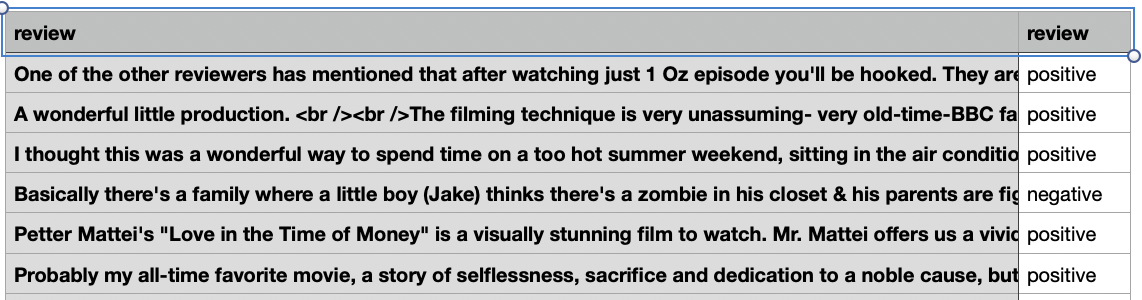
\includegraphics[scale=0.5]{IMDBDataset.png}
	\centering
	\caption{IMDB Dataset}
	\label{fig:imdb_data}
\end{figure}

\section{Results}
% In this section, you will describe and discuss the results of your experiments
% using suitable figures and tables

\subsection{Performance of the models with and without dropout}
Table \ref{tab:loss_train_val_test} shows the mean loss value for multiple models which were trained. A loss of 0 signifies the best sentiment classification.

\begin{table}[h]
	\begin{center}
		\begin{tabular}{c|c|c|c} % <-- Alignments: all columns center
			\textbf{} & \textbf{D=0,Z=0,H=128} & \textbf{D=0,Z=0.1,H=128} & \textbf{D=0.05,Z=0,H=256} \\
			\hline
			Train loss & 0.004, 0.000, 0.036 & 0.011, 0.010 & 0.002, 0.006, 0.005 \\
			Validation loss & 0.344, 0.234, 0.283 & 0.281, 0.262 & 0.249, 0.284, 0.298 \\
			Test loss & 0.572, 0.603, 0.572 & 0.582, 0.504 & 0.533, 0.464, 0.575 \\
		\end{tabular}
		\medskip
		\caption{Mean loss of training, validation and test data sets for the different models. Models are specified by their dropout(D), zoneout(Z) and number of units in hidden layers(H). Multiple loss values are given if training was done multiple times.}
		\label{tab:loss_train_val_test}
	\end{center}
\end{table}

The average train, validation and test losses for various models seem to show that regularization improves performance on test data. For zoneout 0.1 we observed minimum average test loss of 0.504 and for dropconnect 0.05 it was 0.464. Due to the randomness involved in the code, we trained the same model multiple times to see test data performances. But we also notice that better performance on validation data set does not necessarily mean better test data performance. We did not do statistical tests but the observed data indicates that introduction of either of the dropout variants did not produce any significant improvement in the test data performance.

\subsection{Visualizations}

\begin{figure}
	\centering
	\begin{subfigure}[b]{0.22\textwidth}
		\centering
		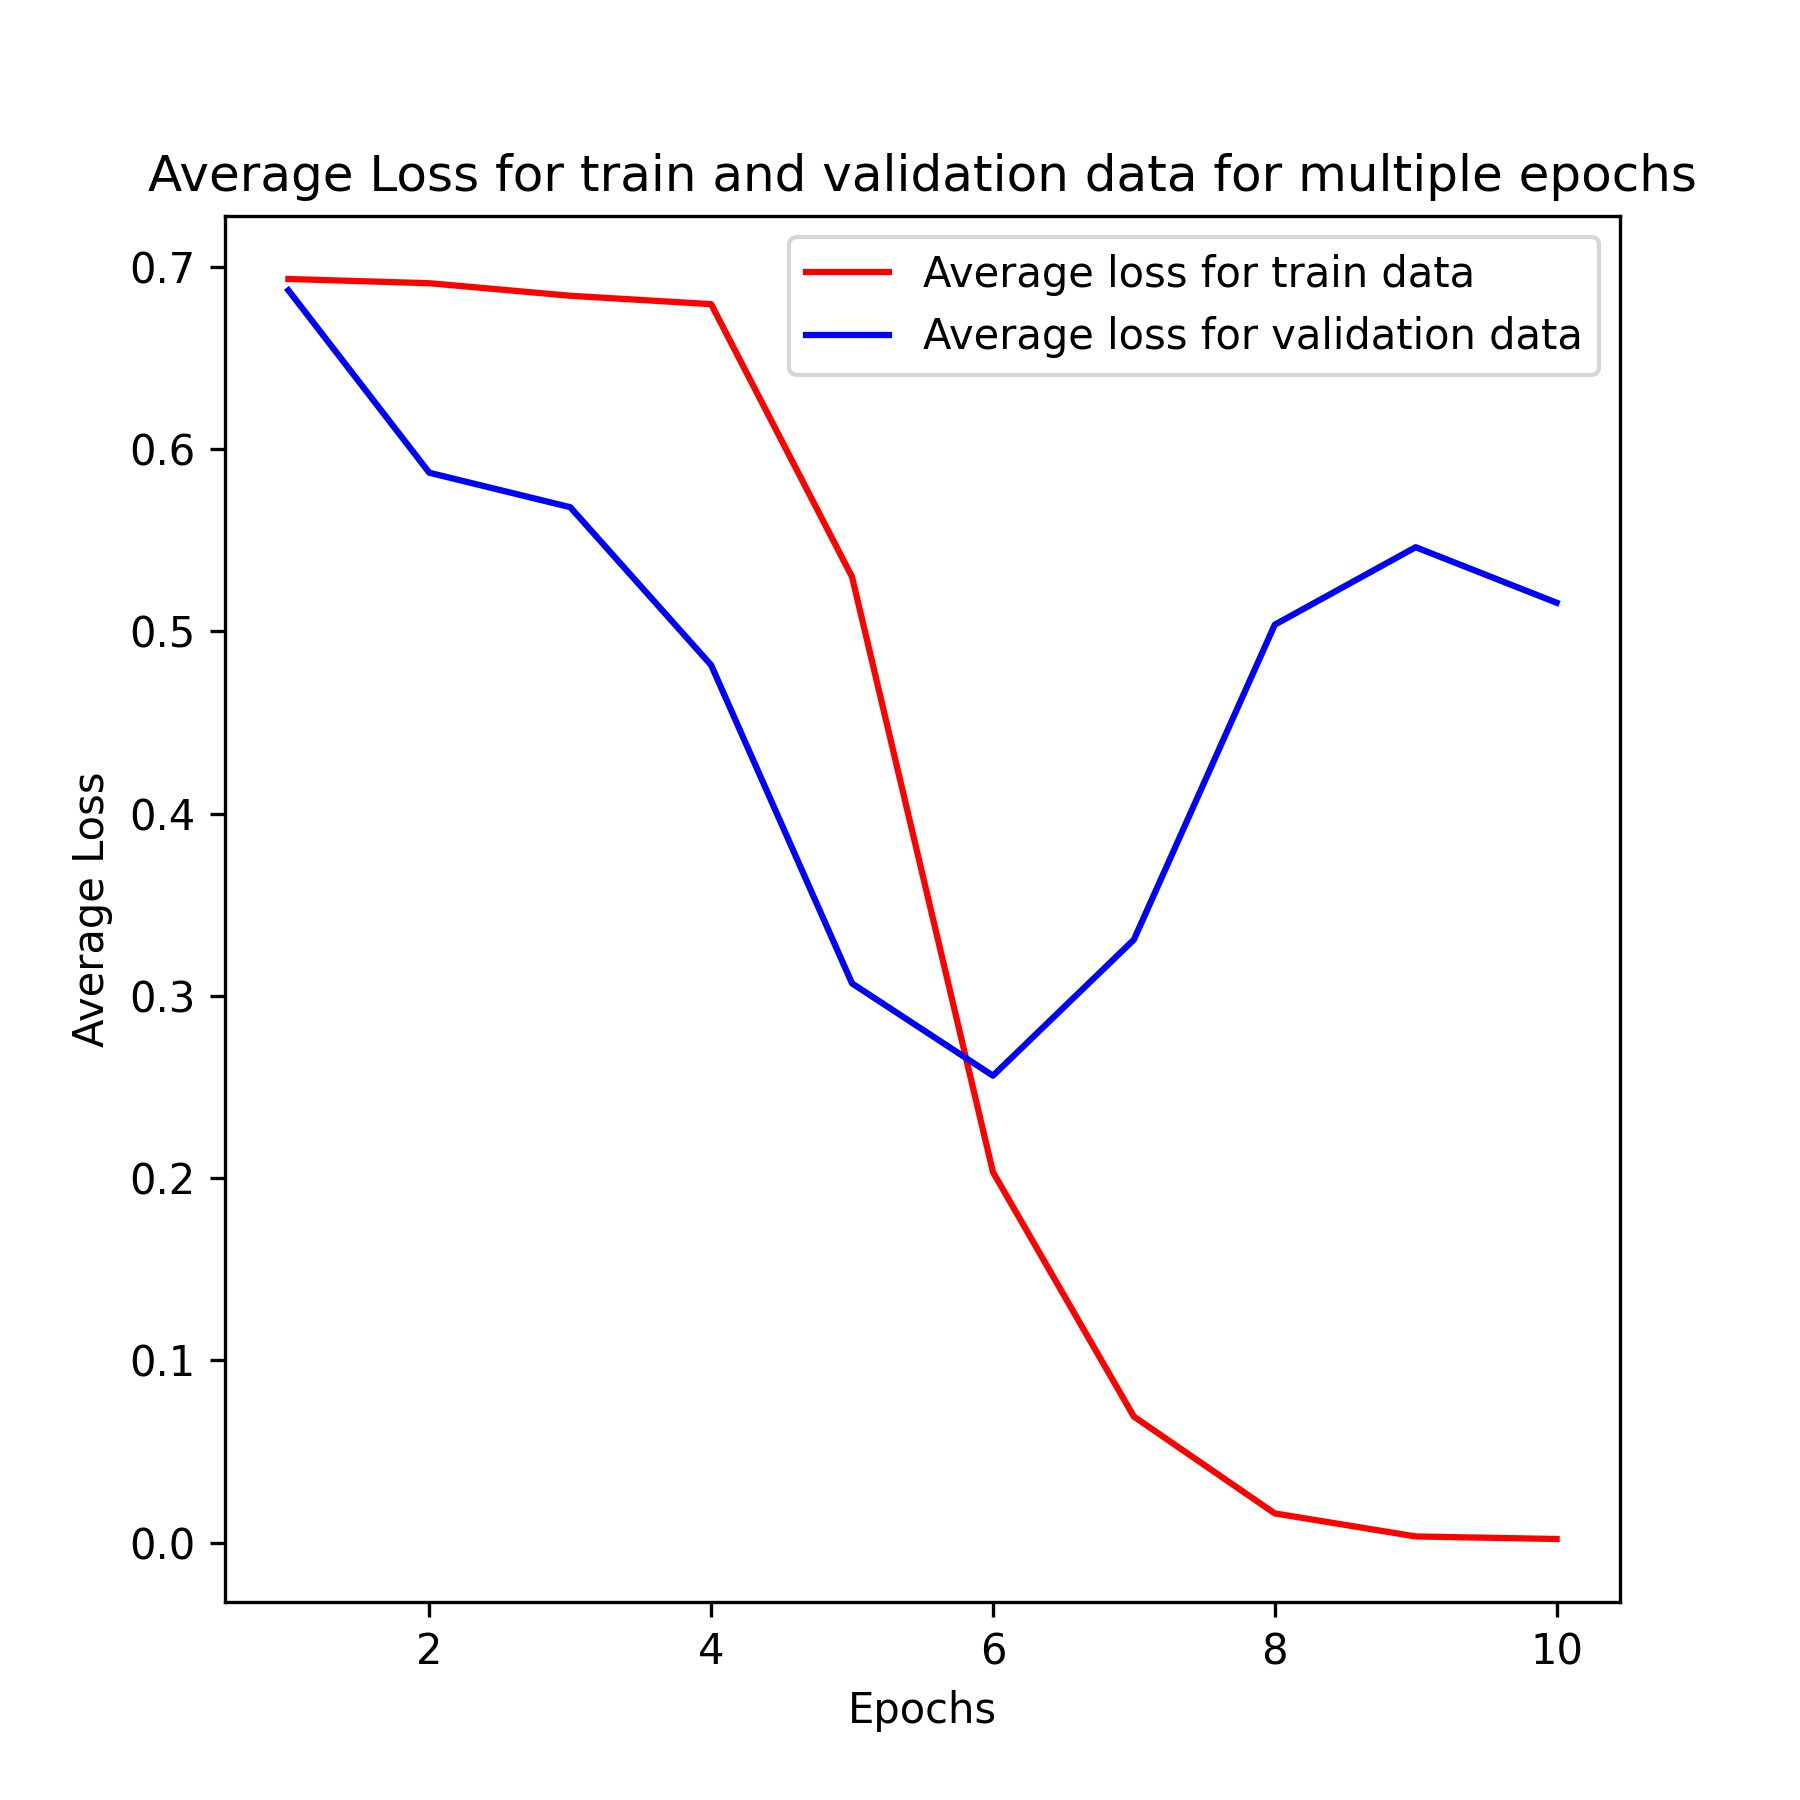
\includegraphics[width=\textwidth]{d0_z0_h128_1D_1.jpg}
		\caption{d0,z0,h128}
	\end{subfigure}
	\begin{subfigure}[b]{0.22\textwidth}
		\centering
		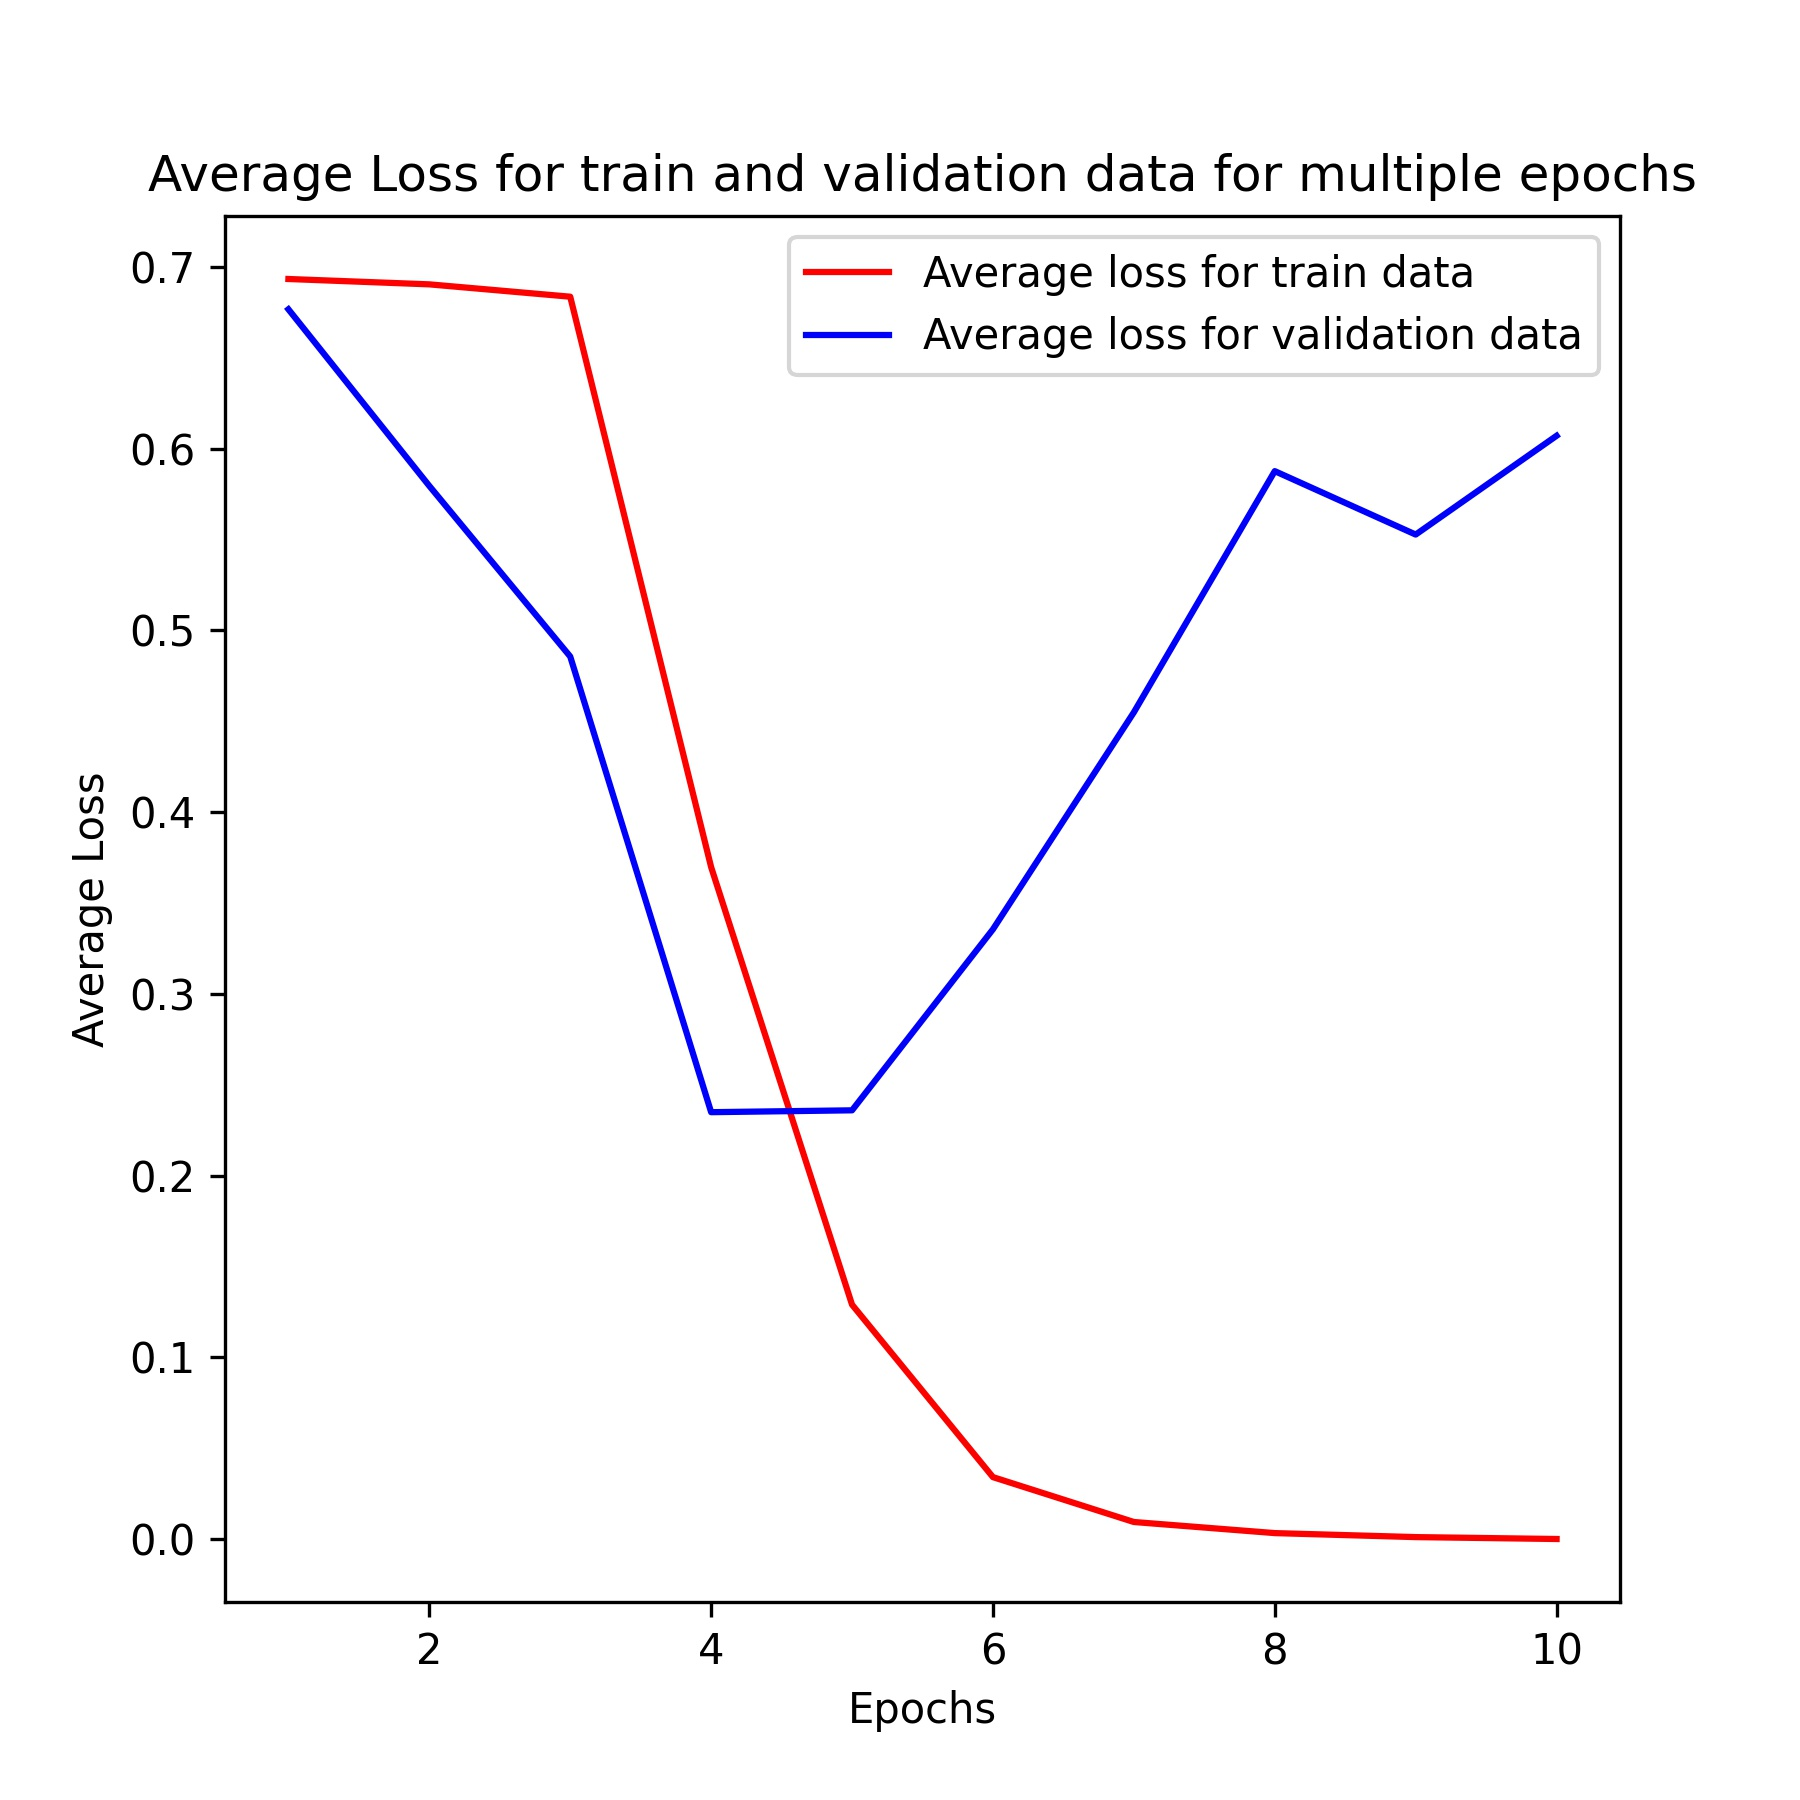
\includegraphics[width=\textwidth]{d0_z0_h128_1D_2.jpg}
		\caption{d0,z0,h128}
	\end{subfigure}
	\begin{subfigure}[b]{0.22\textwidth}
		\centering
		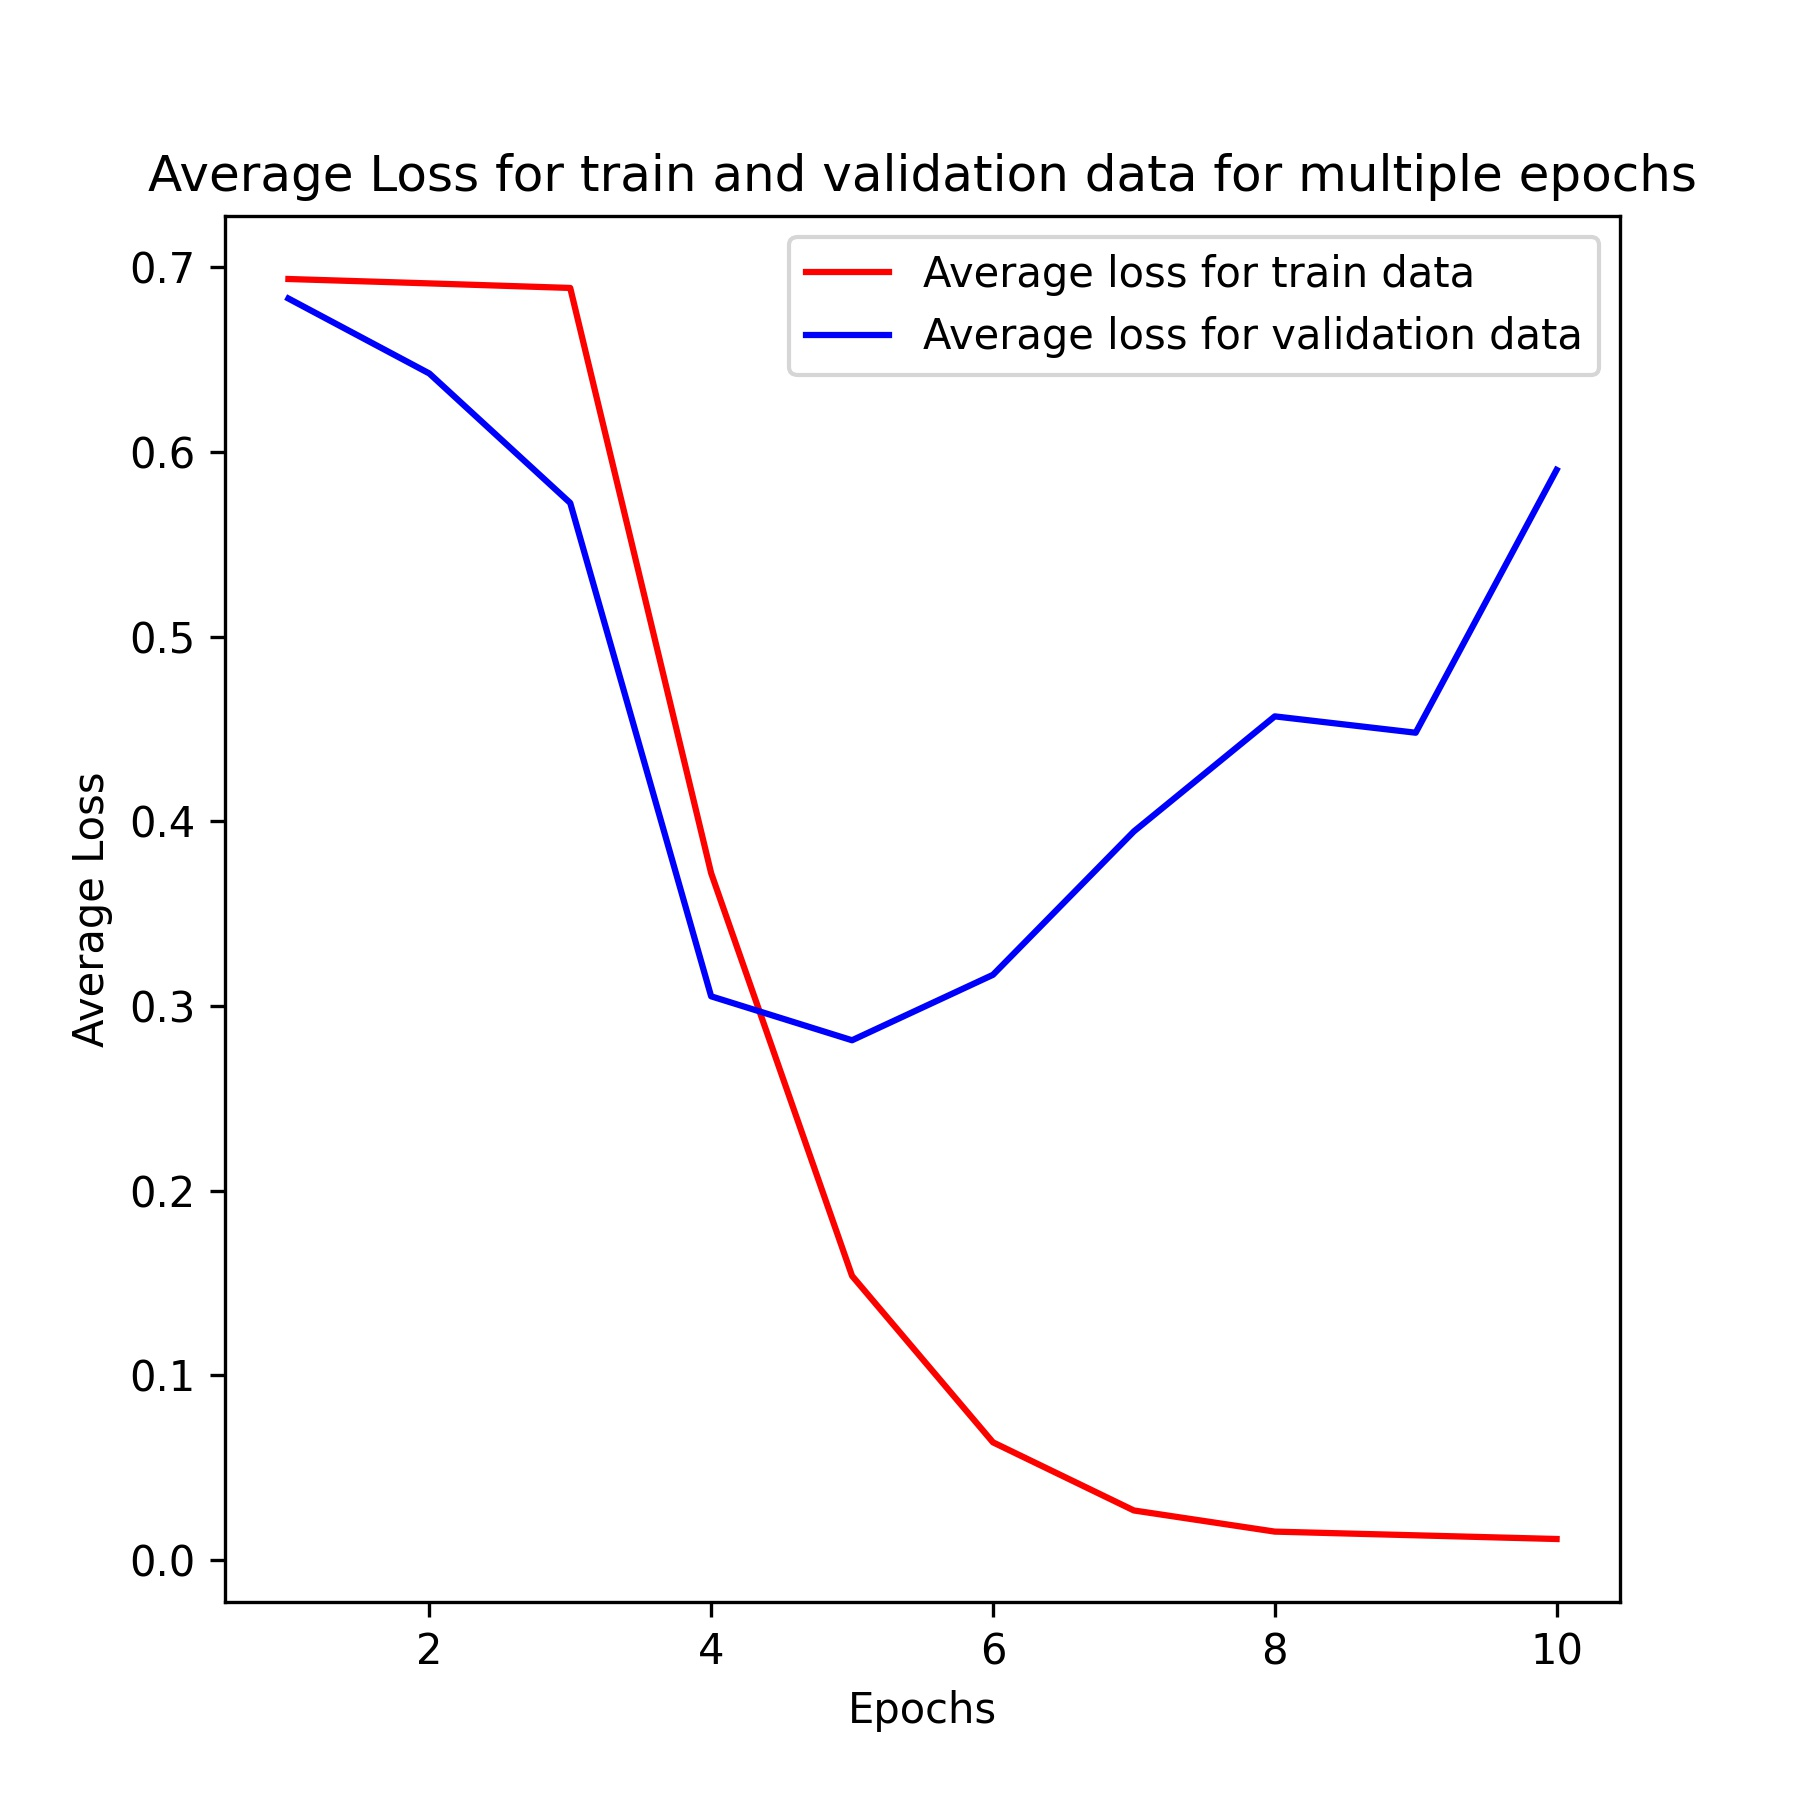
\includegraphics[width=\textwidth]{d0_z0.1_h128_1D_1.jpg}
		\caption{d0,z0.1,h128}
	\end{subfigure}
	\begin{subfigure}[b]{0.22\textwidth}
		\centering
		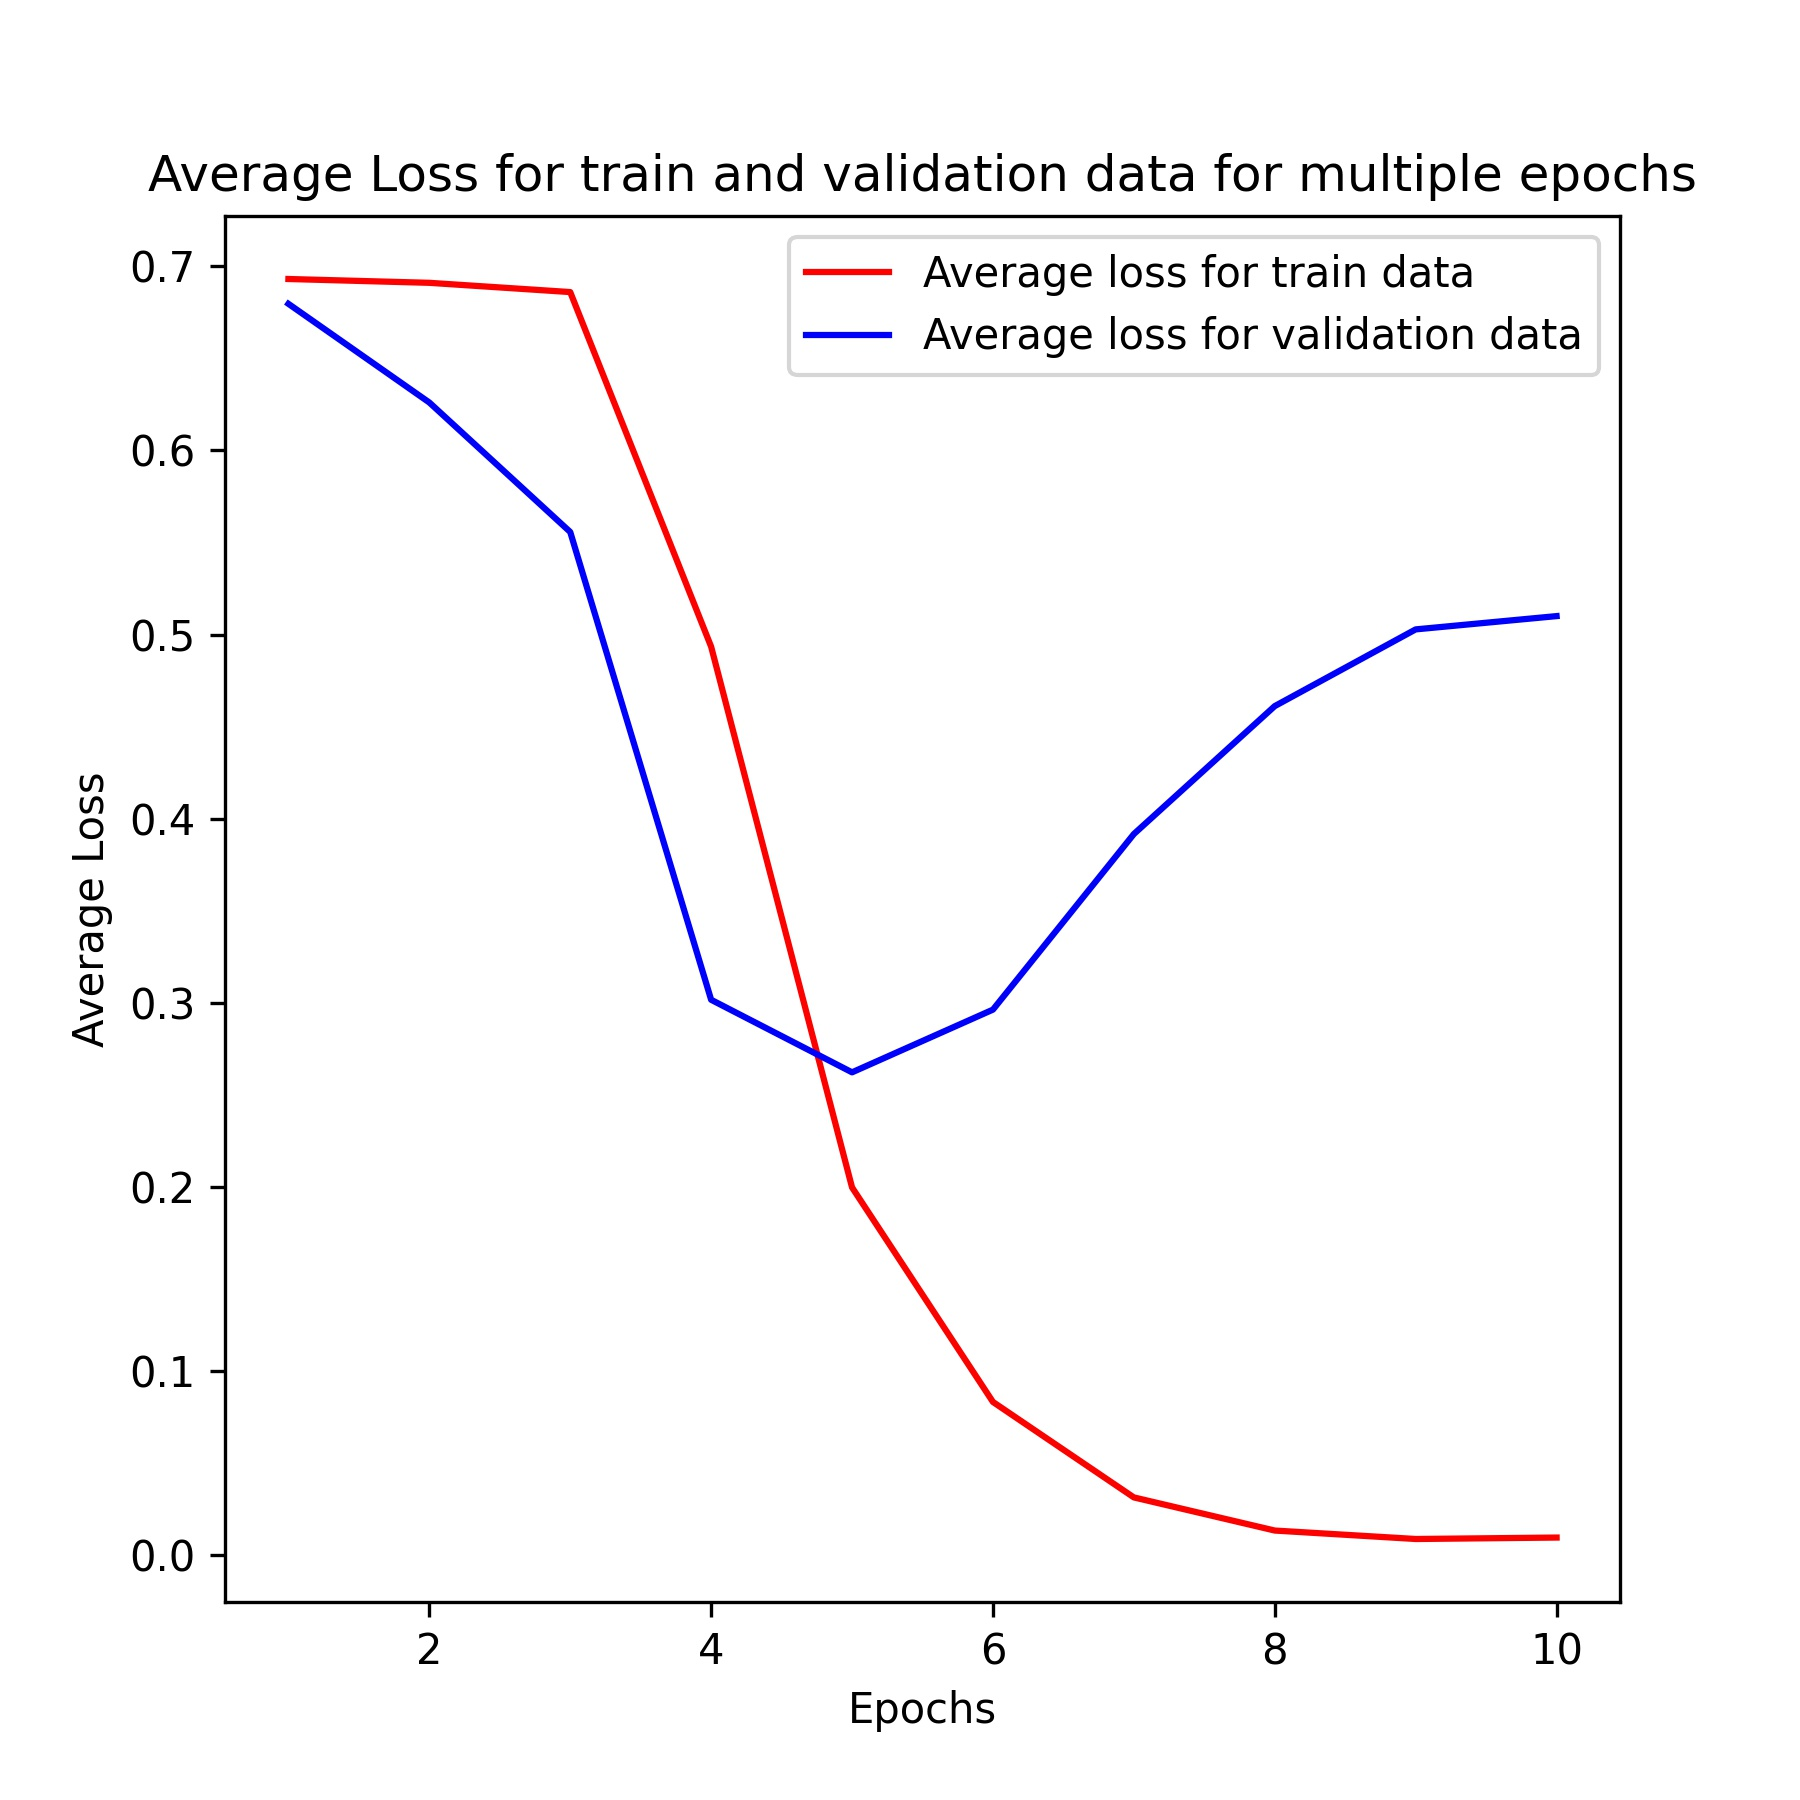
\includegraphics[width=\textwidth]{d0_z0.1_h128_1D_2.jpg}
		\caption{d0,z0.1,h128}
	\end{subfigure}
	\begin{subfigure}[b]{0.22\textwidth}
		\centering
		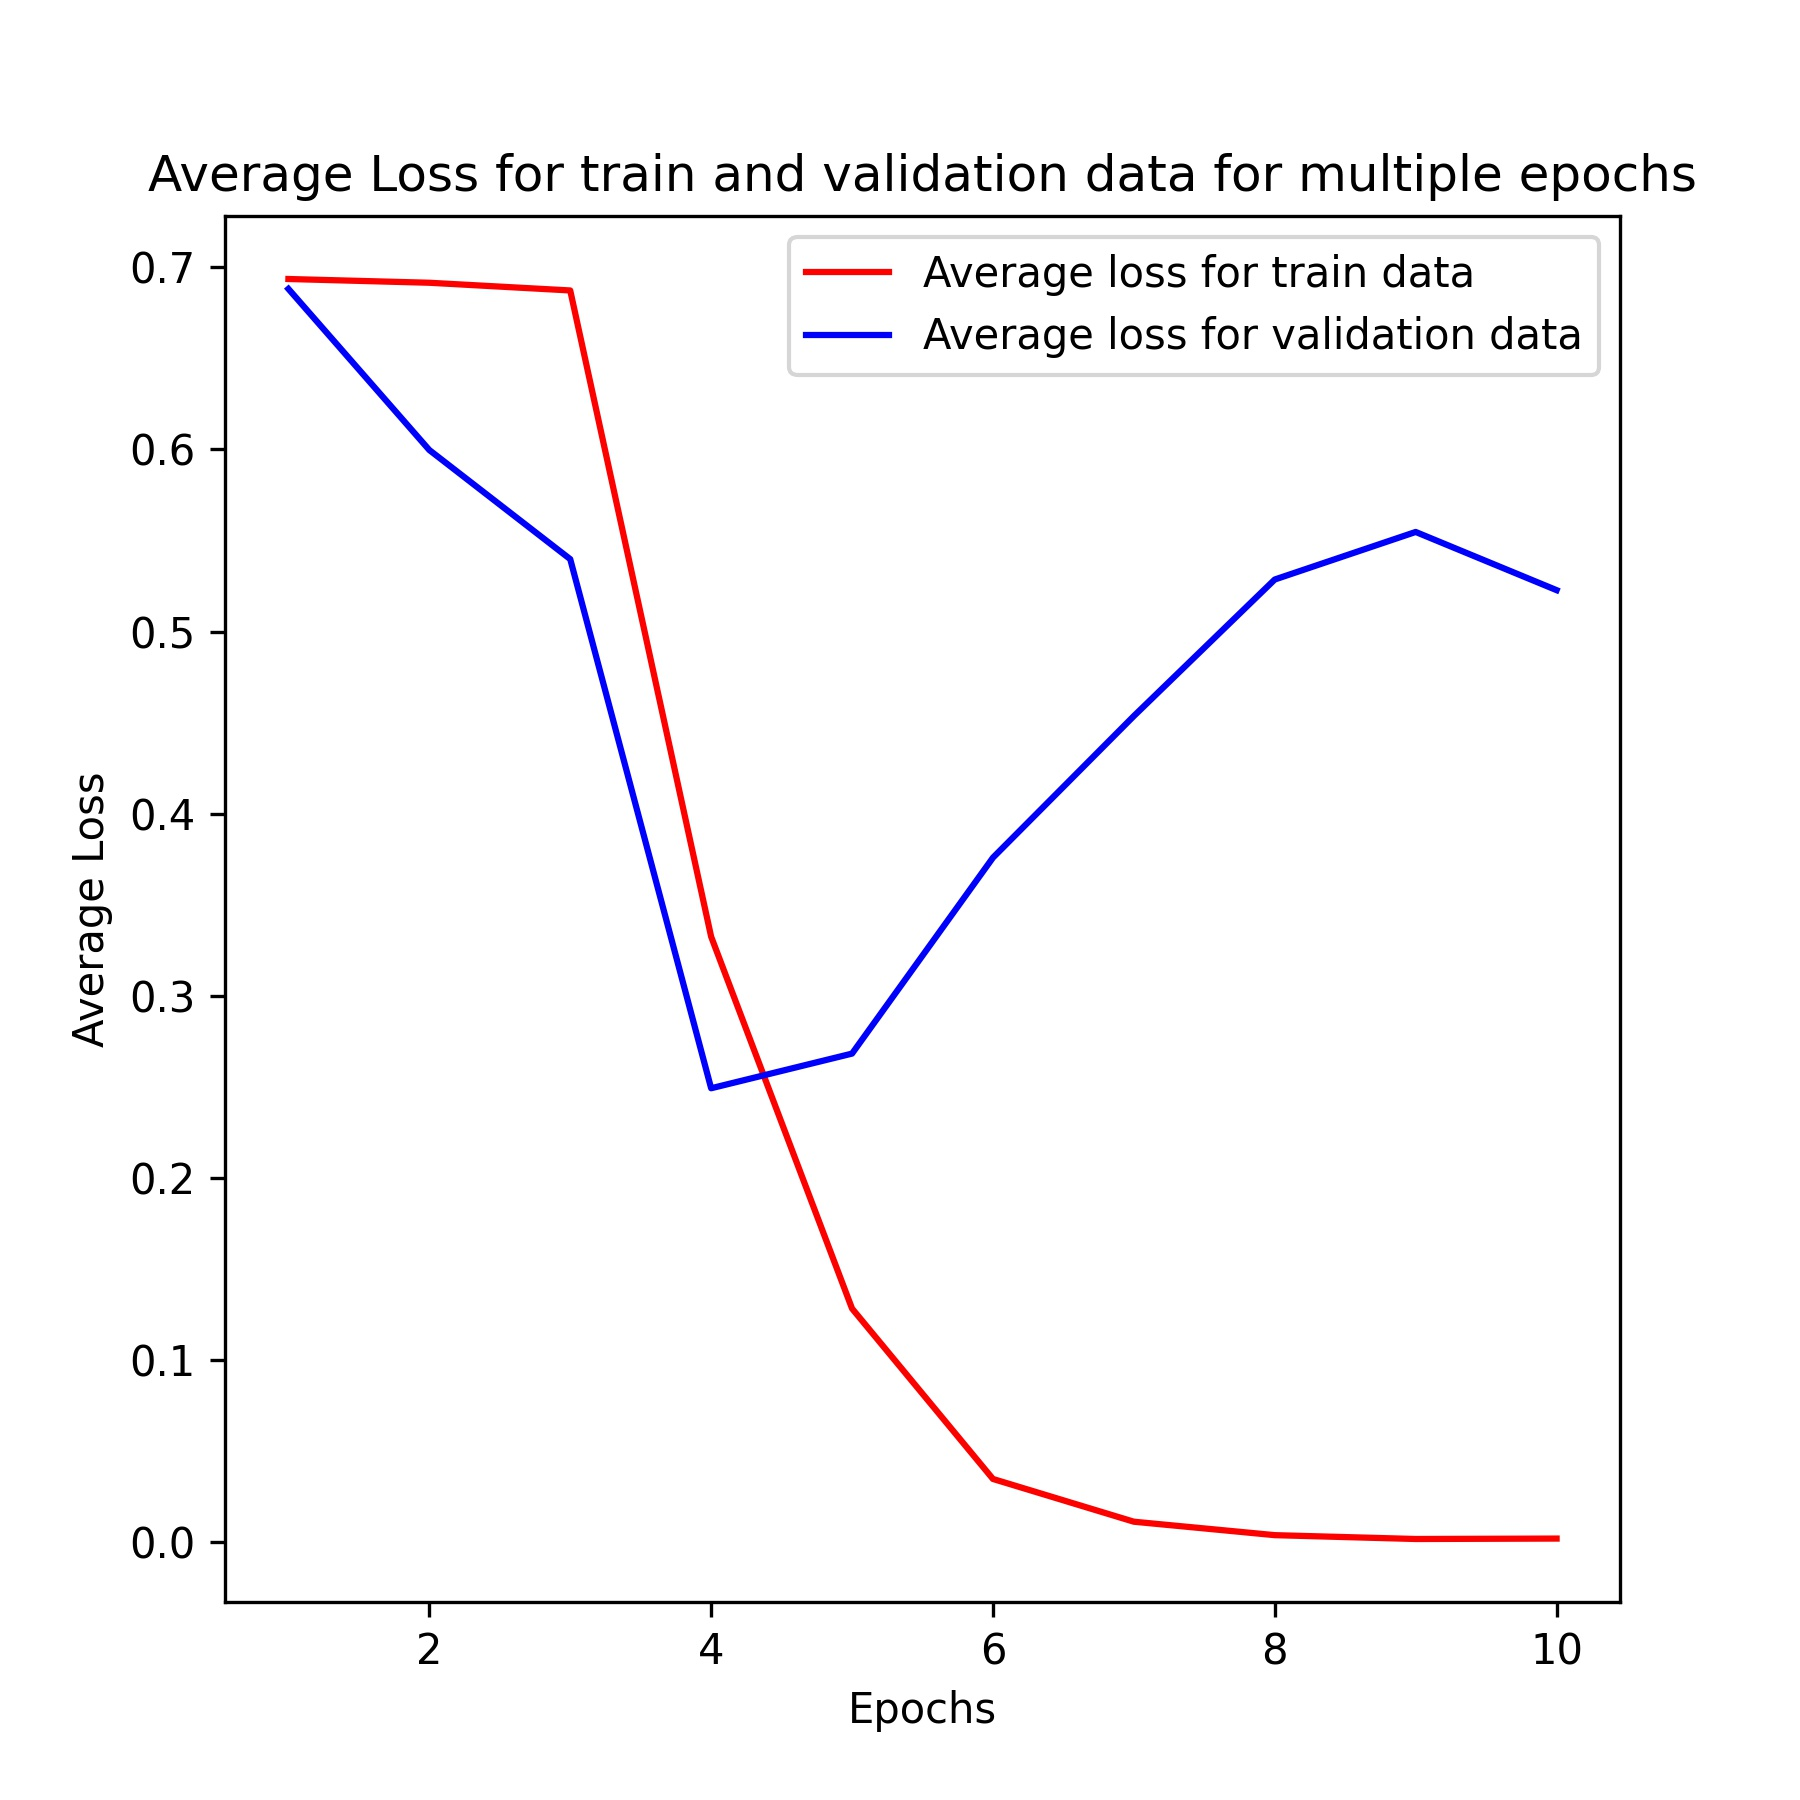
\includegraphics[width=\textwidth]{d0.05_z0_h256_1D_1.jpg}
		\caption{d0.05,z0,h256}
	\end{subfigure}
	\begin{subfigure}[b]{0.22\textwidth}
		\centering
		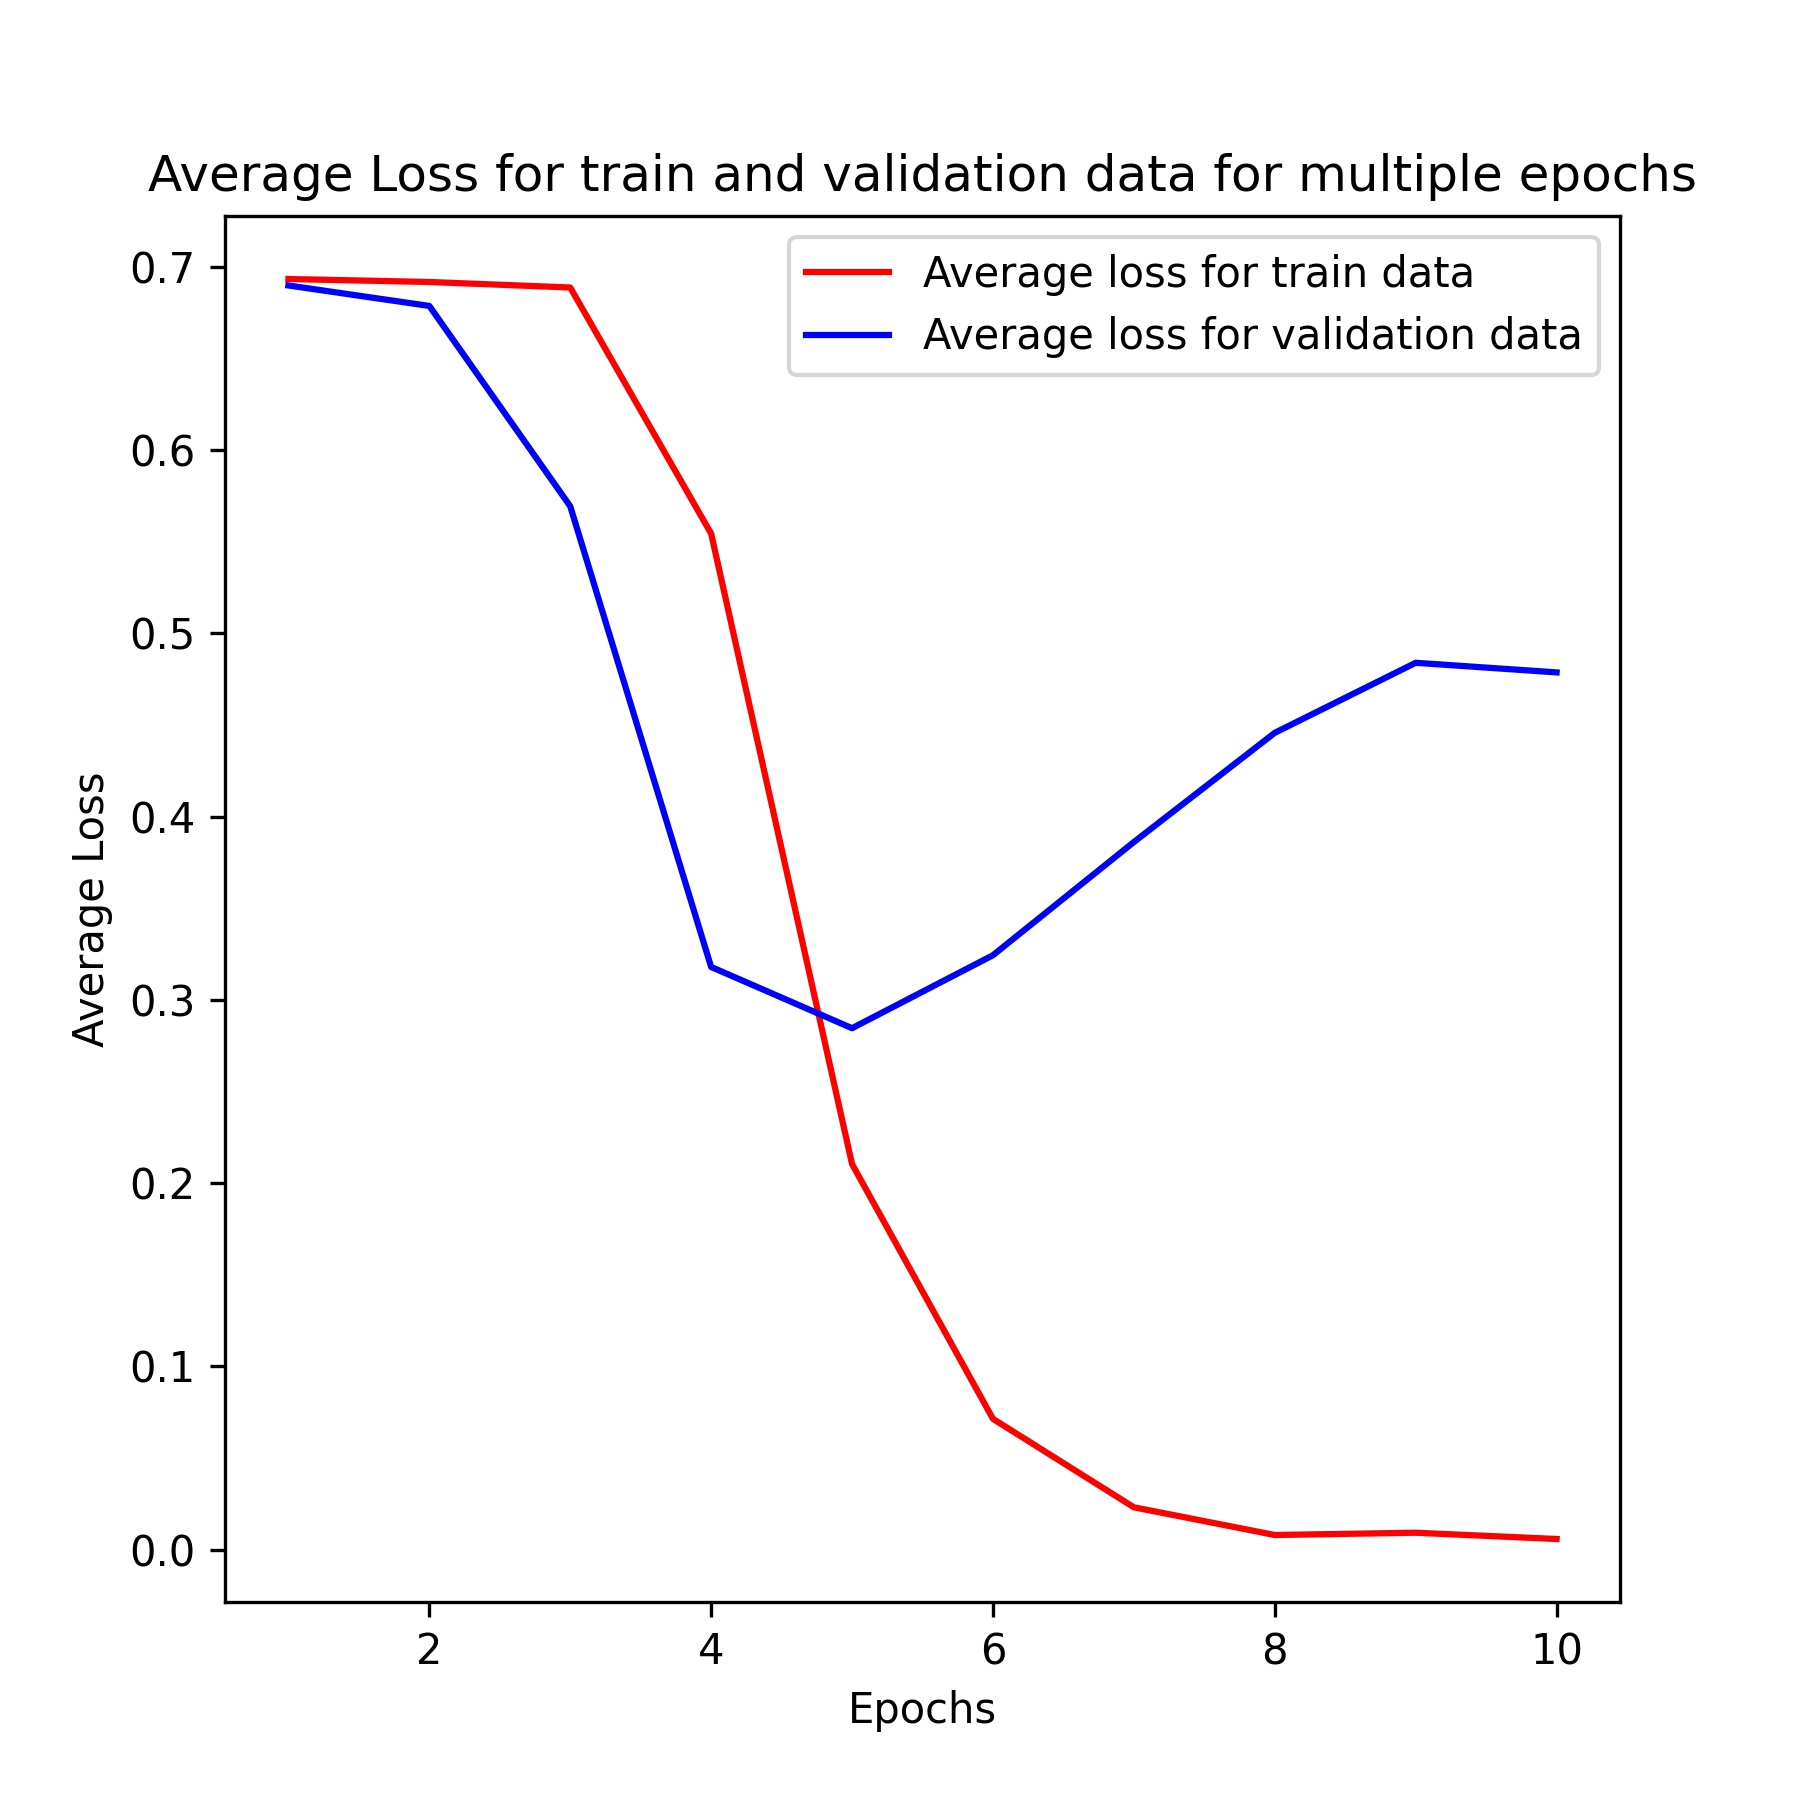
\includegraphics[width=\textwidth]{d0.05_z0_h256_1D_2.jpg}
		\caption{d0.05,z0,h256}
	\end{subfigure}
	\caption{Average loss vs number of epochs for training and validation data for different models. Sub figure caption d$\bf{\alpha}$,z$\bf{\beta}$,h$\bf{\gamma}$ means that the model was being trained with dropconnect ratio $\alpha$, zoneout ratio $\beta$ and $\gamma$ number of units per hidden layer. (a), (b) are for the base model; (c), (d) are for the best zoneout model; and (e), (f) are for the best dropconnect model.}
	\label{fig:loss_epoch_curve}
\end{figure}

Figure \ref{fig:loss_epoch_curve} shows the loss vs number of epochs curves for all the three types of models.

Figure \ref{fig:loss_surface_visualization} shows 2D contour plots and 3D loss surface visualizations for all the three types of models.

The loss vs number of epochs curves are for the same values which are mentioned in the table. We do not see any observable change in the training data convergence rate with and without zoneout/dropconnect. In both cases the model starts overfitting from 5-6 epochs and reaches $\sim$0 average train loss value. As mentioned above, the validation loss also does not show significant improvement with the addition of dropout.


The loss surface visualizations give an indication that the introduction of dropout increases the surface area of the minima in the loss landscape and also makes the path reaching that minima smoother. In figure \ref{fig:loss_surface_visualization}, the contour plots (a) and (b) have more irregularities and the area of minimum loss is smaller. Compared to that, (c) with zoneout has a smoother contour plot and the area of the flat surface is larger. Dropconnect regularization is making the flat surface much larger than both zoneout and no-dropout variants. Increasing the dropconnect ratio from 0.05 to 0.1 clearly increased the flat minima surface. In terms of smoothness, it is perhaps similar to zoneout but better than no-dropout.

Large flat surface in the loss landscape could mean that the model is simplifying the loss function landscape and adding bias, making it easier for the optimizer to reach the minima. This observation is similar to what is seen with ResNets having skip-connections for an image classification problem.

\begin{figure}
    \centering
    \begin{subfigure}[b]{0.3\textwidth}
        \centering
		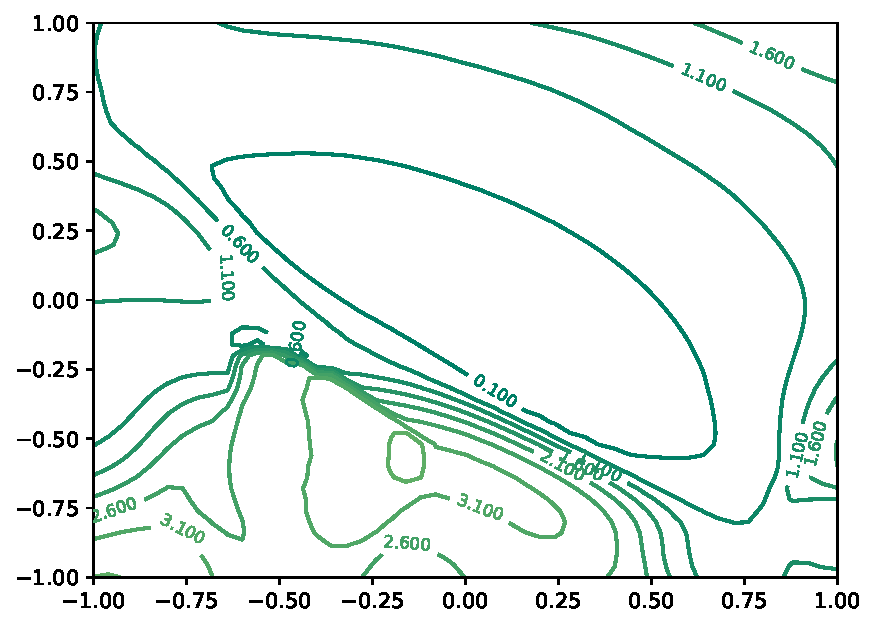
\includegraphics[width=\textwidth]{report_images/d0_z0_h128_2D_1.pdf}
		\caption{d0,z0,h128}
    \end{subfigure}
    \begin{subfigure}[b]{0.3\textwidth}
        \centering
		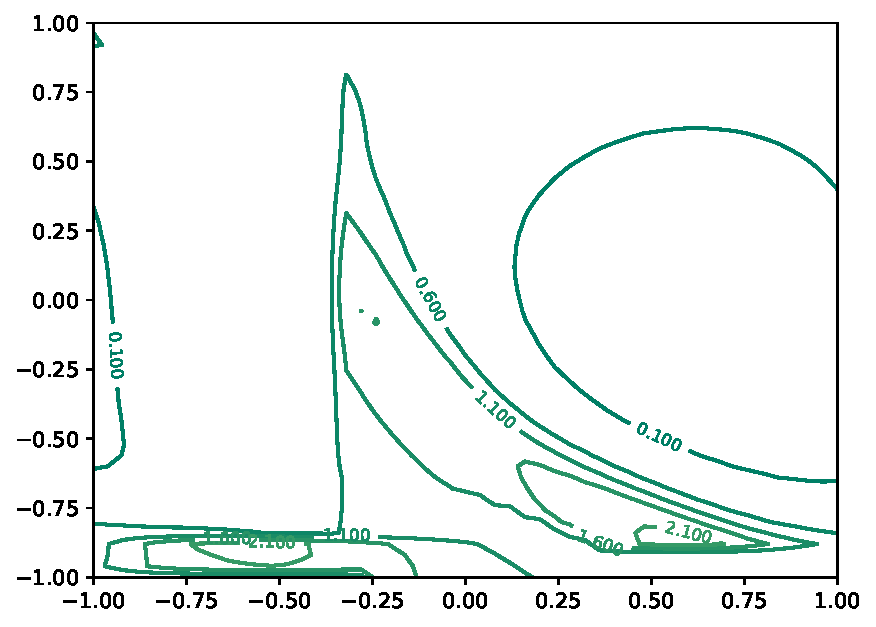
\includegraphics[width=\textwidth]{report_images/d0_z0_h128_2D_2.pdf}
		\caption{d0,z0,h128}
    \end{subfigure}
    \begin{subfigure}[b]{0.3\textwidth}
        \centering
		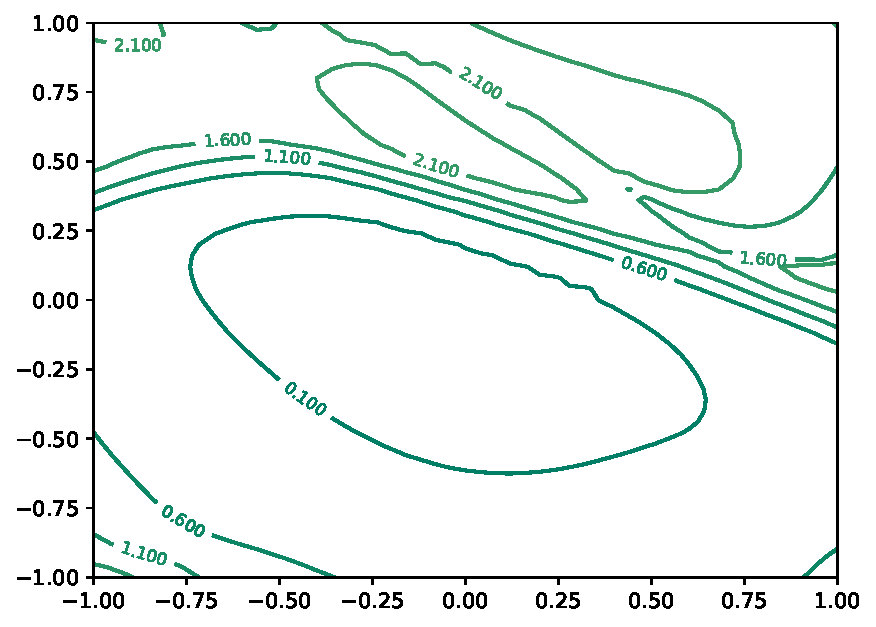
\includegraphics[width=\textwidth]{report_images/d0_z0.1_h128_2D.pdf}
		\caption{d0,z0.1,h128}
    \end{subfigure}
    \begin{subfigure}[b]{0.3\textwidth}
        \centering
		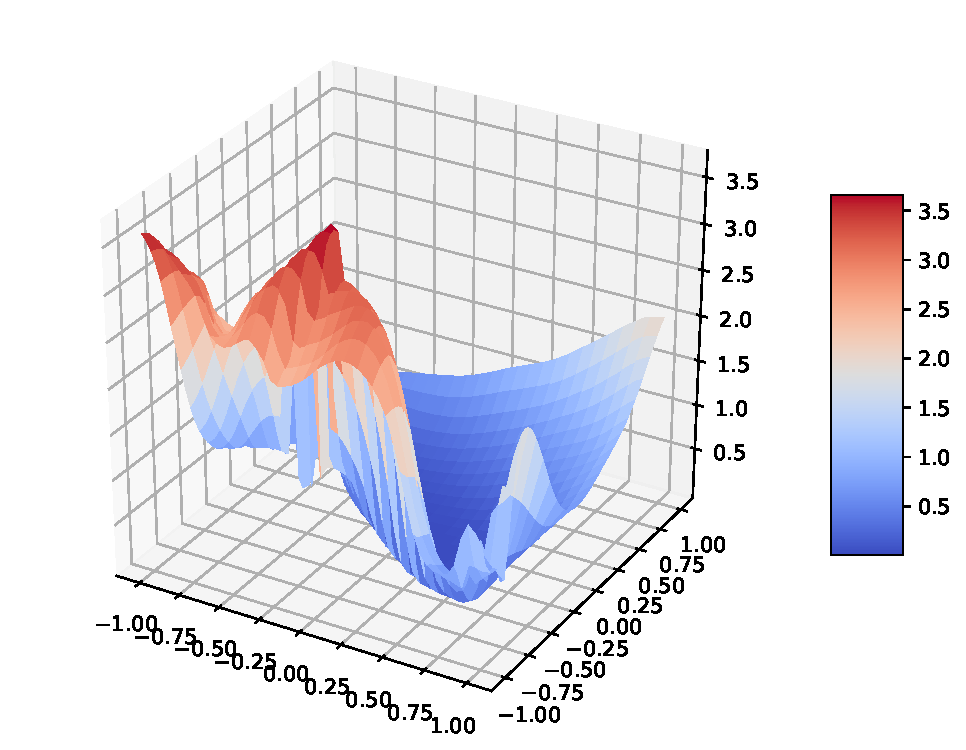
\includegraphics[width=\textwidth]{report_images/d0_z0_h128_3D_1.pdf}
		\caption{d0,z0,h128}
    \end{subfigure}
    \begin{subfigure}[b]{0.3\textwidth}
        \centering
		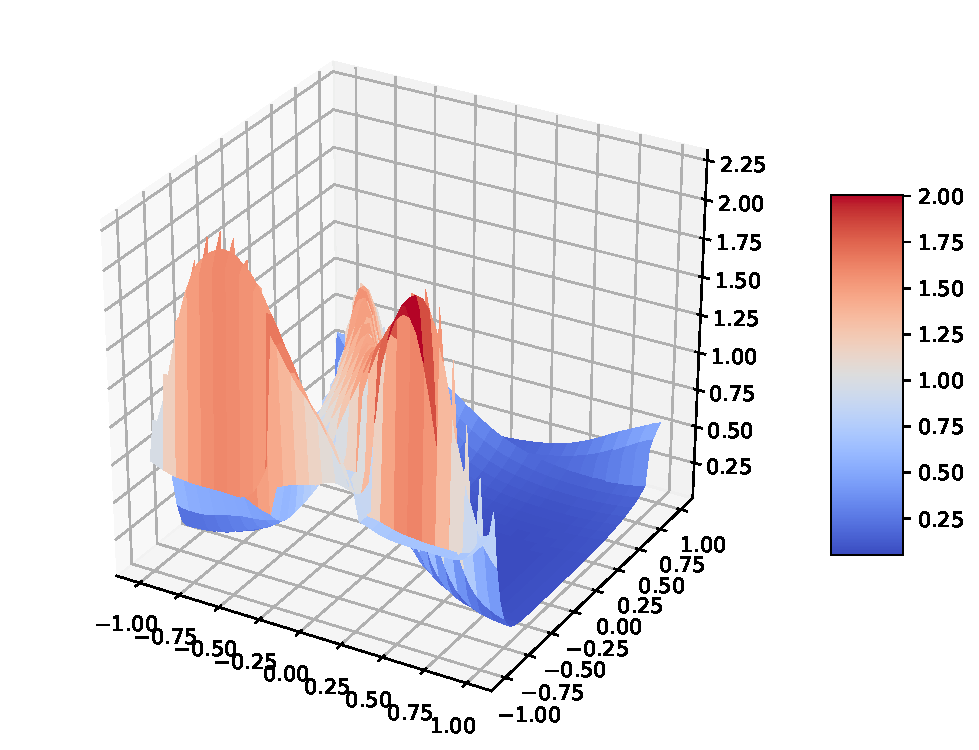
\includegraphics[width=\textwidth]{report_images/d0_z0_h128_3D_2.pdf}
		\caption{d0,z0,h128}
    \end{subfigure}
    \begin{subfigure}[b]{0.3\textwidth}
        \centering
		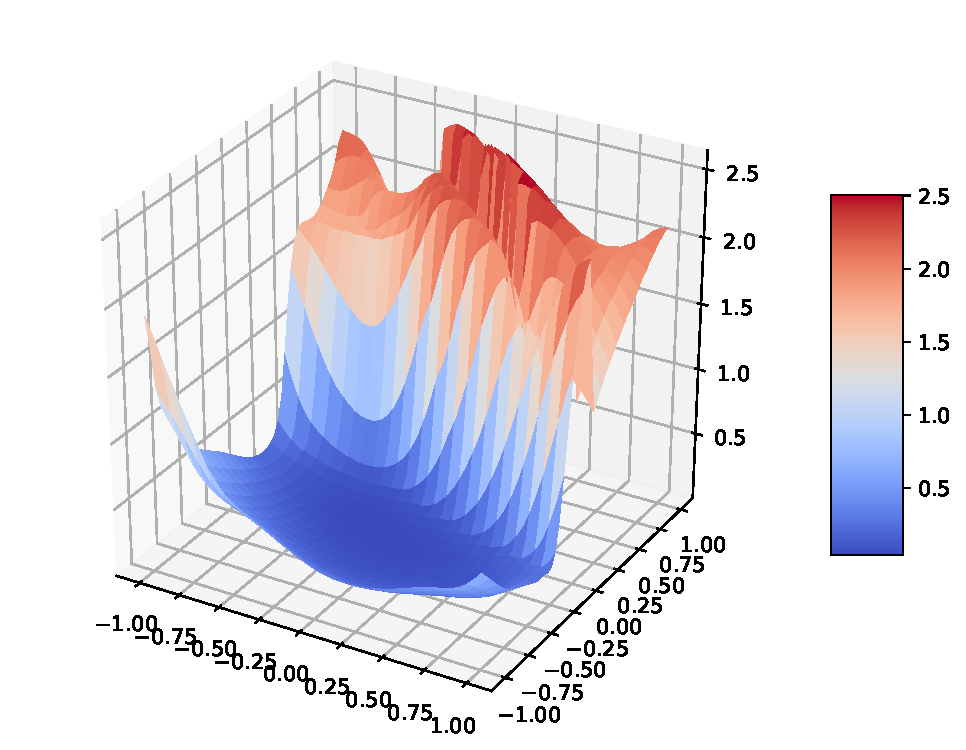
\includegraphics[width=\textwidth]{report_images/d0_z0.1_h128_3D.pdf}
		\caption{d0,z0.1,h128}
    \end{subfigure}
    \begin{subfigure}[b]{0.3\textwidth}
        \centering
		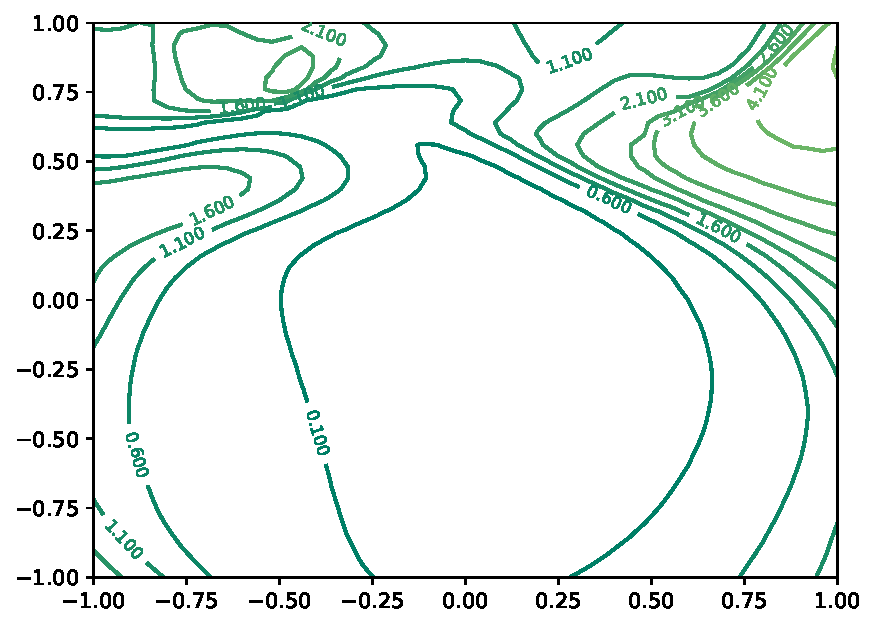
\includegraphics[width=\textwidth]{report_images/d0.05_z0_h256_2D.pdf}
		\caption{d0.05,z0,h256}
    \end{subfigure}
    \begin{subfigure}[b]{0.3\textwidth}
        \centering
		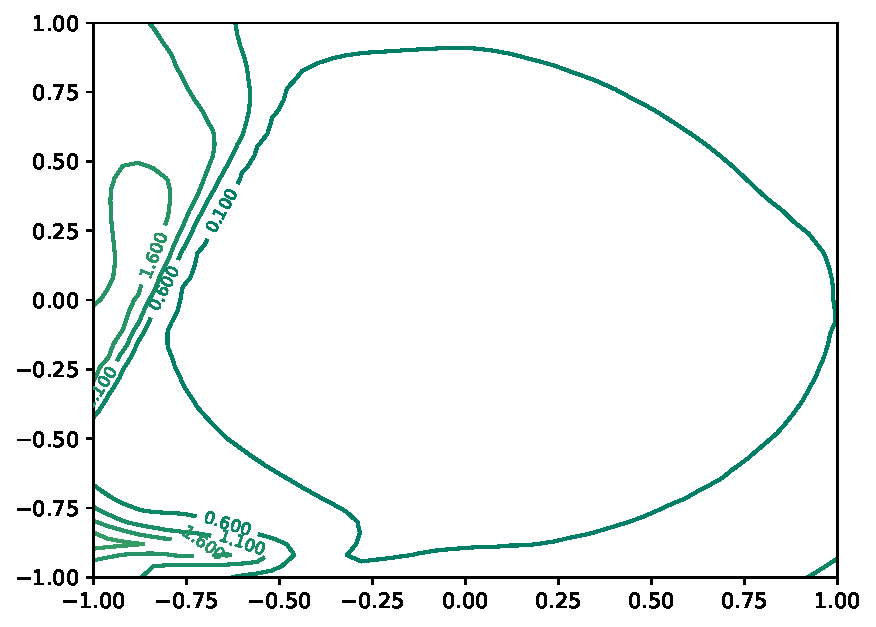
\includegraphics[width=\textwidth]{report_images/d0.1_z0_h256_2D.pdf}
		\caption{d0.1,z0,h256}
    \end{subfigure}
    % leaving a blank line changes the row for the next subfigure
    
    \begin{subfigure}[b]{0.3\textwidth}
        \centering
		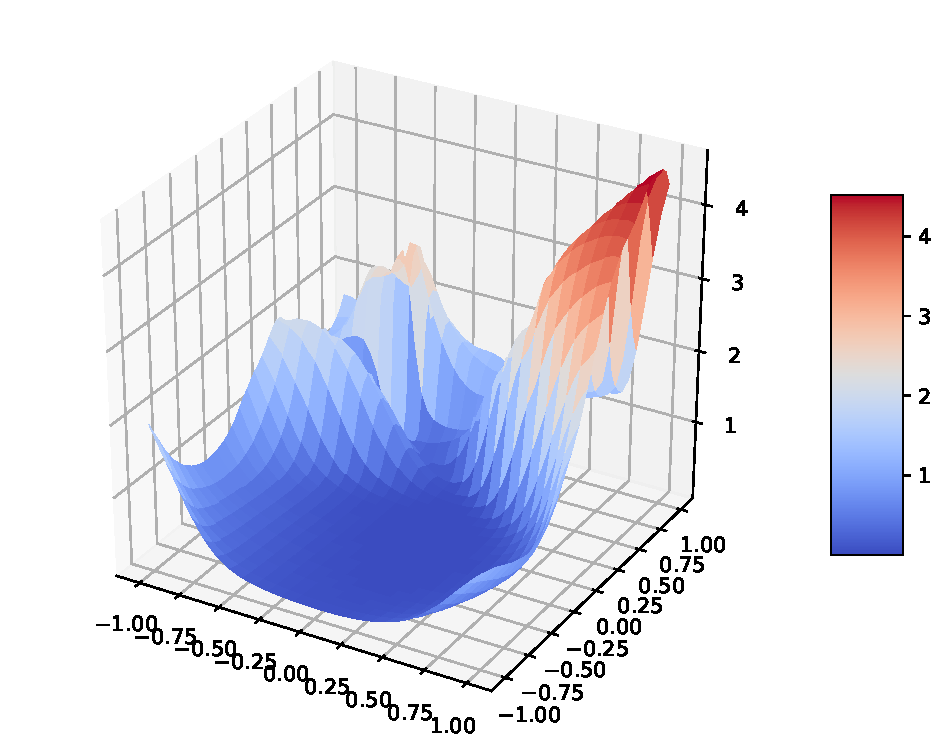
\includegraphics[width=\textwidth]{report_images/d0.05_z0_h256_3D.pdf}
		\caption{d0.05,z0,h256}
    \end{subfigure}
    \begin{subfigure}[b]{0.3\textwidth}
        \centering
		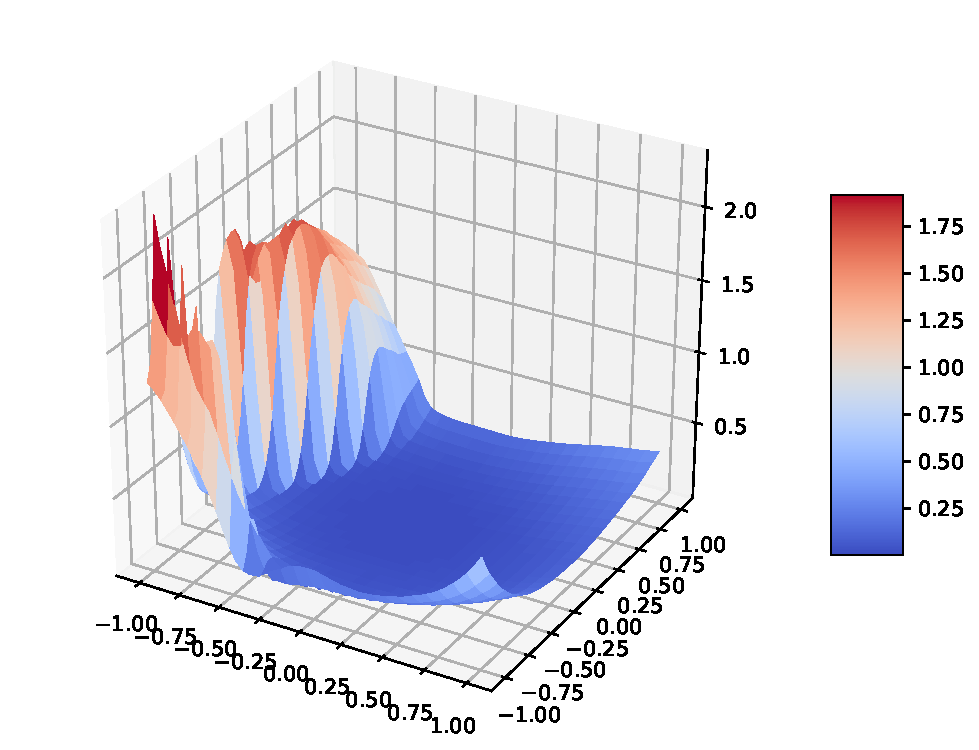
\includegraphics[width=\textwidth]{report_images/d0.1_z0_h256_3D.pdf}
		\caption{d0.1,z0,h256}
    \end{subfigure}
    \caption{2D and 3D loss surface visualizations for different models. Sub figure caption d$\bf{\alpha}$,z$\bf{\beta}$,h$\bf{\gamma}$ means that the model was being trained with dropconnect ratio $\alpha$, zoneout ratio $\beta$ and $\gamma$ number of units per hidden layer. Sub figures are arranged in pairs for easier correlation between figures. a-d, b-e, c-f, g-i, h-j represent the same loss surfaces in 2D and 3D formats.}
    \label{fig:loss_surface_visualization}
\end{figure}

\subsection{Adversarial Test Inputs}
% R
We performed two main experiments to check the robustness of our models with respect to adversarial inputs. 
\subsubsection{Evaluating our best models with adversarial inputs}
In the first experiment (Table \ref{tab:exp1}), we evaluated all three of our models(No dropout, Zoneout=0.1, DropConnect=0.05) with the 200 adversarial inputs. We see that the model trained with DropConnect fares better than the model without dropout and the model with Zoneout. This proves that the model trained with DropConnect variant is robust to adversarial examples, which is our hypothesis. This is not happening for our Zoneout model and we believe the DropConnect model, by dropping hidden-hidden weights, is regularizing more compared to the Zoneout model which still retains the previous layer activations.
\begin{table}[h]
	\begin{center}
		\begin{tabular}{c|c} % <-- Alignments: all columns center
			\textbf{} & \textbf{Test Loss} \\
			\hline
			No dropout & 1.208\\
			Zoneout=0.1 & 1.353\\
			DropConnect=0.05 & 0.544\\
		\end{tabular}
		\medskip
		\caption{Average losses for out best models with adversarial test inputs.}
		\label{tab:exp1}
	\end{center}
\end{table}

\subsubsection{Evaluating our best models with adversarial inputs by applying Dropout at test time}

In this experiment, we applied dropout at test time(Table \ref{tab:exp2}) expecting each model to fare better at evaluating the adversarial examples. We found that to be the case with DropConnect, as we see lesser loss for the model at test time with dropconnect. This was again not seen in the case of Zoneout because we believe that Zoneout may not be as high a regularizer as compared to DropConnect for this input.

\begin{table}[h]
	\begin{center}
		\begin{tabular}{c|c|c} % <-- Alignments: all columns center
			\textbf{} & \textbf{Zoneout=0.1} & \textbf{DropConnect=0.05}\\
			\hline
			With dropout at Test time & 1.365 & 0.537\\
			Without dropout at Test time & 1.353 & 0.544\\
		\end{tabular}
		\medskip
		\caption{Evaluating our best models with adversarial inputs by applying Dropout at test time}
		\label{tab:exp2}
	\end{center}
\end{table}

\section{Discussion and Conclusions}
% In this section, you will discuss the overall
% outcomes of your project. How do your results relate to what has been reported in the
% literature previously? What seemed to work well and what didn’t? Did you run into any
% particular problems? What else would you have done if you had more time? What
% should others learn from your results?

Through our experiments, we satisfactorily showed that the introduction of zoneout and dropconnect increases the surface area having the minimum loss function value and it also makes the path reaching that area smoother. This result is similar to what was observed by \cite{li2018visualizing} for image classification models DenseNet, and ResNet-56 using skip-connection regularization.

This should naturally have resulted in faster convergence of training data but we did not see much changes in that aspect. We also did not observe significant performance improvements in the test data predictions. All models successfully fit the training data giving 97-100\% accuracy in predictions. This indicates that the dataset was not complex enough to observe the regularization impacts. Perhaps using a tougher dataset would have shown faster convergence and different test accuracy. It's not clear whether the test performance for such a dataset would have improved or not.

In our experiments involving adversarial inputs, we see that for models with DropConnect, using dropout at both training time and test time significantly improves the model performance. Also, we notice that models trained with Dropconnect perform better than the baseline model and zoneout model on regular test data. This is akin to the related literature on vanilla dropout but both these results don't hold true for Zoneout. We believe the DropConnect model, by dropping hidden-hidden weights, is regularizing more in comparison to the Zoneout model which still retains the previous layer activations. Our view is that, the larger degree of regularization is making the DropConnect model more robust to adversarial inputs in contrast to the Zoneout model. 

The 2D and 3D visualizations were very resource intensive and required 9+ hours of runtime on google colab's single GPU instance. This limitation prevented us from trying multiple visualizations at various hyperparameter values to understand the effects in a better way. The code had to be written in a very robust way, adding checkpoints and saving parameters after every epoch or any significant computation, so as to account for sudden notebook run failures and disconnection issues. Producing adversarial examples using TextAttack was also very time consuming even though we found ways to parallelize the code using multiple cores.

Given more time, we would have tried out one more datasets which is complex enough to show visible improvements/degradation with the addition of dropout. We would have also liked to explore a dataset for which Zoneout would give a better performance than DropConnect. We would have tried to build a model for multi-class, multi-label document classification problem (for e.g. using Reuters dataset) which would have more evaluation criteria compared to binary sentiment classification. With more compute, we would have generated more 2D/3D plots, some during hyperparameter tuning, to notice how the loss landscape looks when we choose a bad HP combination (high zoneout, high dropconnect, less hidden units). When it comes to the adversarial examples it would have been interesting to try out different kinds of attacks on our Dropout variants to see whether they are able to generalize over various attacks. We would have also liked to see how adversarial training can be combined with dropout to make the model more robust.



\bibliographystyle{apalike}
\footnotesize
\bibliography{yourbib}

\end{document}
